%% A simple template for a lab or course report using the Hagenberg setup
%% with the standard LaTeX 'report' class
\documentclass[english,11pt]{report}		
%\documentclass[ngerman,11pt]{report}
\usepackage{hyperref}
\usepackage{hgb}
\usepackage{hgbbib}
\usepackage{hgbheadings}
\usepackage{array,booktabs}
\usepackage[export]{adjustbox}
\usepackage{tabu}
\usepackage{pdfpages}
\usepackage{caption}
\usepackage{float}
\usepackage[version=4]{mhchem}
\usepackage{chronology}
\usepackage[topmargin=.5 in]{geometry}
\graphicspath{{images/}}   % where are the images?
\bibliography{literatur}  % requires literatur.bib 
\title{\huge{Study of the Electrical system of the new Power and Blowing Station II}\\[.4em]
\small{and}\\[.4em]
\huge{Emergency calculations for power requirements in case of power failure} \\[1em] 
\Large{Anshul Dubey (2015A3PS309H)} \\
\Large{Himanshu Gupta (2015A3PS339H)} \\
\Large{Mihir Kumar (2015B3A3564H)} \\
\Large{Salil Jain (2015B5A3578G)} \\
[2em] \large{Final Report submitted in partial fulfillment for\\
Practice School I (BITS F221)\\[1em]
under the guidance of\\[.3em]}
\Large{Mr. V.S. Dewangan}\\[.8em]
\large{Submitted to}\\[.3em]
\Large{Prof. Ashutosh Bhatia}}
\date{$7^{th}$ July 2017}

% \lhead{
\includegraphics[width=1cm]{bits123.png}}
% \lhead{
\includegraphics[width=1.5cm]{sail123.png}}
%%%----------------------------------------------------------
\begin{document}
%%%----------------------------------------------------------
\maketitle

\chapter*{\centering Preface}
\textit{``The trick to having good ideas is not to sit around in glorious isolation and try to think big thoughts. The trick is to get more parts on the table.''}

\begin{flushright}
-Steven Johnson
\end{flushright}
If a picture is worth thousand words then a face to reality is priceless. \\[1em]
Project provides an engineer one such opportunity to explore the practical aspects of one’s technical knowledge apart from giving a firsthand experience to the professional work environment and opportunity to meet the strong technical work force.\\[1em]
We would like to thank everyone concerned for their time, enthusiasm and effort. Bhilai Steel Plant provided all the data needed for the project.\\[1em]
The project report focuses on the Study of the Electrical system of the new Power and Blowing Station II (PBS-II) and the Emergency calculations for power requirements in case of power failure.\\[1em]
Finally, we regret any inadvertent errors that might have crept in. We hope that reading these proceedings is joie-de-vivre.\\

\chapter*{\centering Acknowledgement}
In preparing these proceedings we have been fortunate to receive valuable guidance, kind support, suggestions, inspiration and assistance from our guide and his colleagues. We greatly appreciate their generosity in devoting their valuable time to help us in pursuing this project.\\[1em]
t is with feelings of profound thankfulness and deep sense of gratitude that we acknowledge the invaluable guidance and consistent encouragement rendered to us by \textbf{Mr. V. S. Dewangan (AGM, PP-I)}, Bhilai Steel Plant (SAIL), India. He spared valuable time from his busy schedule for us and helped us by guiding for the project. Our sincere thanks to \textbf{Mr. Dewangan} for all the help and resources that were made available to us.\\[1em]
We are deeply indebted to our PS Instructor\textbf{ Mr. Ashutosh Bhatia} for his constant assistance and help in facilitating and organising the various activities regarding the Summer Internship.\\[1em]
We would also like to thank our Project Mentor \textbf{Dr. G.R. Sabareesh} for his valuable input regarding the project.\\[1em]
We are also thankful to\textbf{ Mr. V.M. Rao, Pankaj Rathore} and all the respected individuals who were directly or indirectly involved in the successful completion of our Technical project.


\chapter*{\centering Declaration}
We hereby declare that project work entitled \textbf{“Study of the Electrical system of the new Power and Blowing Station II and Emergency calculations for power requirements in case of power failure.”} is an authentic record of our own work carried out at the Power and Blowing Station (PBS-2) of Bhilai Steel Plant under the supervision of Mr. V.S. Dewangan and the guidance of Mr. Ashutosh Bhatia, during 22nd May 2017 to 15th July 2017. \\[2em]
Anshul Dubey\\[.5em]
Himanshu Gupta \\[.5em]
Mihir Kumar \\[.5em]
Salil Jain \\[3.5em]
Date : $7^{th}$ July 2017

\chapter*{\centering Certificate}
\begin{center}

\includegraphics[width = 2in]{sail123.png}
\end{center}
This is to certify that report entitled \textbf{“Study of the Electrical system of the new Power and Blowing Station II and Emergency calculations for power requirements in case of power failure.”}, which is submitted by  Anshul Dubey, Himanshu Gupta, Mihir Kumar and Salil Jain pursuing B.E. (Hons.) at BITS Pilani University is a record of candidates own work carried out by them under my supervision. The matter embodied in this project is original and has not been submitted for the award of any other degree. \\[2em]
\begin{flushright}
Shri V.S. Dewangan\\ 
(Assistant General Manager)\\ 
Power and Blowing Station SAIL-BSP
\end{flushright}

\tableofcontents


\chapter{Project Overview}

\section{What is the project about?}

\begin{itemize}
\item To study of all electrical and mechanical system of PBS-2
\item Calculation of the emergency power requirement of different units of PBS-2.
\item Identification of the source of power in BSP to ensure emergency supply in case of power failure.
\end{itemize}

\section{Objective and Significance of the project}

\begin{itemize}
\item Detailed exposure of various process involved in power generation system in steel industry.
\item Function of boilers , DM water plant ,cooling water pump house , cooling towers , turbine, generator for power requirement in any industry .
\item Learning of the various control systems in power plant operations .
\item Role of SCADA  in electrical control system and communication.
\item Calculation of the emergency power requirements of the new Power and Blowing Station II which is being installed in BSP 
\item Power generation from waste heat of COB-11 is also envisaged in this project and 4 MW along with process steam is being utilized in BSP.
\item Total electrical system of BSP are interlinked with PBS-2 for reliable operation of power system in case of power failure
\end{itemize}

\pagebreak
\section{Learning outcomes and Expected Knowledge gain and Deliverable from the project}
% \markboth{}{}
\begin{itemize}
\item Exposure to all electrical system in power industry like generator reactor HT breaker  , LT breaker transformer  cable sizing etc. 
\item Detailed study of SLD for power requirement in any industry 
\item Project management for execution of any project 
\item Commissioning methodology of electrical system 
\item Power calculation of any upcoming unit for reliable operation of plant 
\item Exposure to power plant operation with detailed knowledge of each equipment
\item Introduction to DCS, PLC, SCADA for future references
\end{itemize}


\section{Site Map}
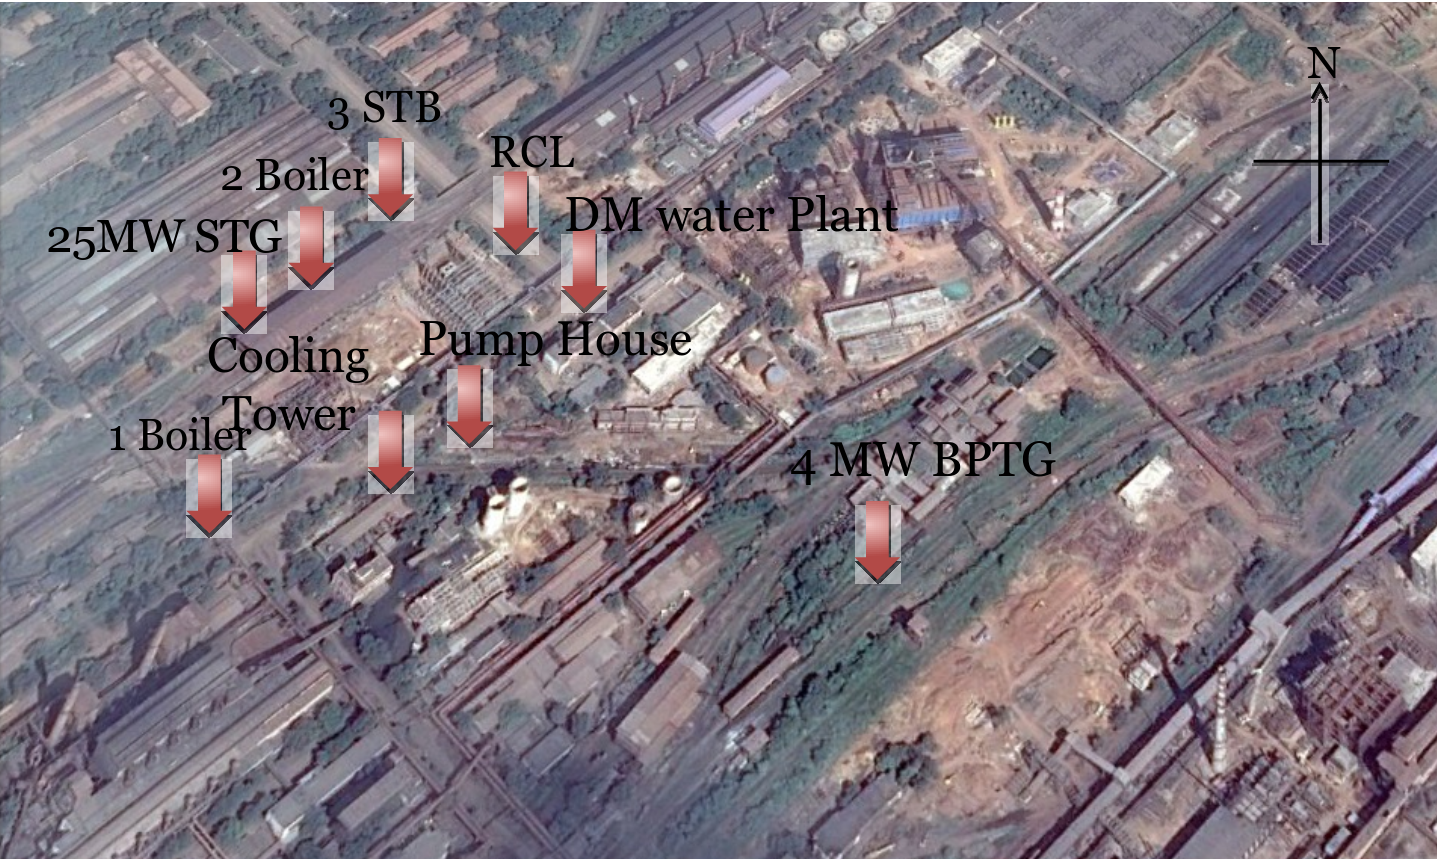
\includegraphics[width =6in]{siteimg.png}

\section{Project Packages}
\begin{center}
\begin{tabu}to 0.8\textwidth { | X[l] | X[l] | X[l] | X[l]|} 
\hline
Package & Installation & Contractors & Contract signing date \\
\hline
011-01-A & 3 Boilers and its auxiliaries. STB Building along with EOT crane  & M/s Fujian Longking Corporation Ltd. and M/s Allied Engineering Services Pvt. Ltd. & 24.03.12\\
\hline
011-01-B & 25 MW STG, 4 MW BPTG, Cooling Tower, Pump House & M/s Triveni Engineering and Industries Ltd.,Banglore & 19.01.12\\
\hline
011-01-C & 3X 225 M3 /Hr. DM water Plant & M/s TechnoFab Engineering Ltd., New Delhi
 & 25.02.12 \\
\hline
12 & 3 STB's and its auxiliaries. & Bharat Heavy Electricals Ltd. & 11.11.10\\
\hline
\end{tabu}
\end{center}

\chapter{Power and Blowing Station-2}
Power & Blowing Station is a vital installation. It serves the following needs of the Bhilai Steel Plant.
\begin{itemize}
    \item Supplying air blast to Blast furnaces at requisite parameters.
    \item Meeting emergency power requirements of the 2.5 MT units of Bhilai Steel Plant in case of any grid power failure and also to generate power to reduce dependency on bought out power and save costs.
    \item Meeting the process steam needs of various shops for their safe/efficient operation.
    \item Buffer consumer of available Blast furnace and coke oven gasses to prevent their wastage/high pressure in the gas line network. As such the shop is required to be run at a high level of efficiency and reliability to ensure that working of other shops particularly Blast furnace are not effected.
\end{itemize}

While P&BS 1 doesn’t use cooling tower in order to cool the “cooling water” at  elevated temperature after absorbing the latent heat of vaporization of steam and works on simple water recycling system PP2 is proposed to have a cooling tower with the  following specifications:
\begin{itemize}
    \item Four pumps of 6.6KV  rated voltage and  55Amps. Actual current to be run with a motor of 540KW capacity, the total energy consumption per hour being 1659.82KWhr.
    \item Five cooling fans of 440V rated voltage and  110 Amps. Actual current to be run with a motor of 74KW capacity
    \item The total energy consumption per hour being 276.6KWhr
    \item Thus the total energy consumption  increased per hour for installing cooling tower at  PP-2 is 1936.45KWhr.
    \item  Though the energy consumption for installing CT at PP-2 would increase in spite of that we would be  save a lot of energy as the cooling water avg. temp. would decrease and thus cycle efficiency would increase as per the formula
    $$\eta = 1 - T_2/T_2$$
    \textbf{As per our study replacing the CT of PP-2 with Indirect Air cooling with Direct Contact Condenser would save 5.35 million M3 water  and  158.30 million rupees  per year!!!}
\end{itemize}
\section{Need of Steam Turbo Blowers in BSP}
Blast Furnaces can be considered as the heart of a Steel Plant. The blast furnace is the first step in producing steel from iron oxides. The purpose of a blast furnace is to chemically reduce and physically convert iron oxides into liquid iron called "hot metal". The raw materials such as iron ore, coke and limestone are dumped into the top and preheated air known as Hot air blast is blown into the bottom. The raw materials undergo numerous chemical reactions and descend to the bottom to become final product of liquid iron and slag. The hot air blast is produced by passing cold air blast trough a stove where residual blast furnace gases are burned. This cold air blast is provided by Turbo blowers form Power and Blowing Station. \\
Each blower installed on the new Power and Blowing station will provide on average 1500 $Nm^{3}/min$ of cold air blast. There will be 3 Steam Turbine driven Turbo Blowers (2 working and 1 Standby) each with 50\% capacity of maximum air blast requirement.\\
\section{Plant Requirement}
\begin{tabular}{|p{3cm}|p{3cm}|p{3cm}|p{3cm}|}
\hline
    \textbf{Requirements} & \textbf{Emergency Power} & \textbf{Air Blast} & \textbf{Process Steam}\\ \hline
    Facility & STG(25 MW), BPTG (4MW) & STG & Boiler (150TPH), BPTG (4 MW)\\ \hline
    Customer & Critical Loads of Plant & Blast Furnace - 8 & Plant Stream \\ \hline
\end{tabular}
\section{Single Line Diagram of PBS-2}
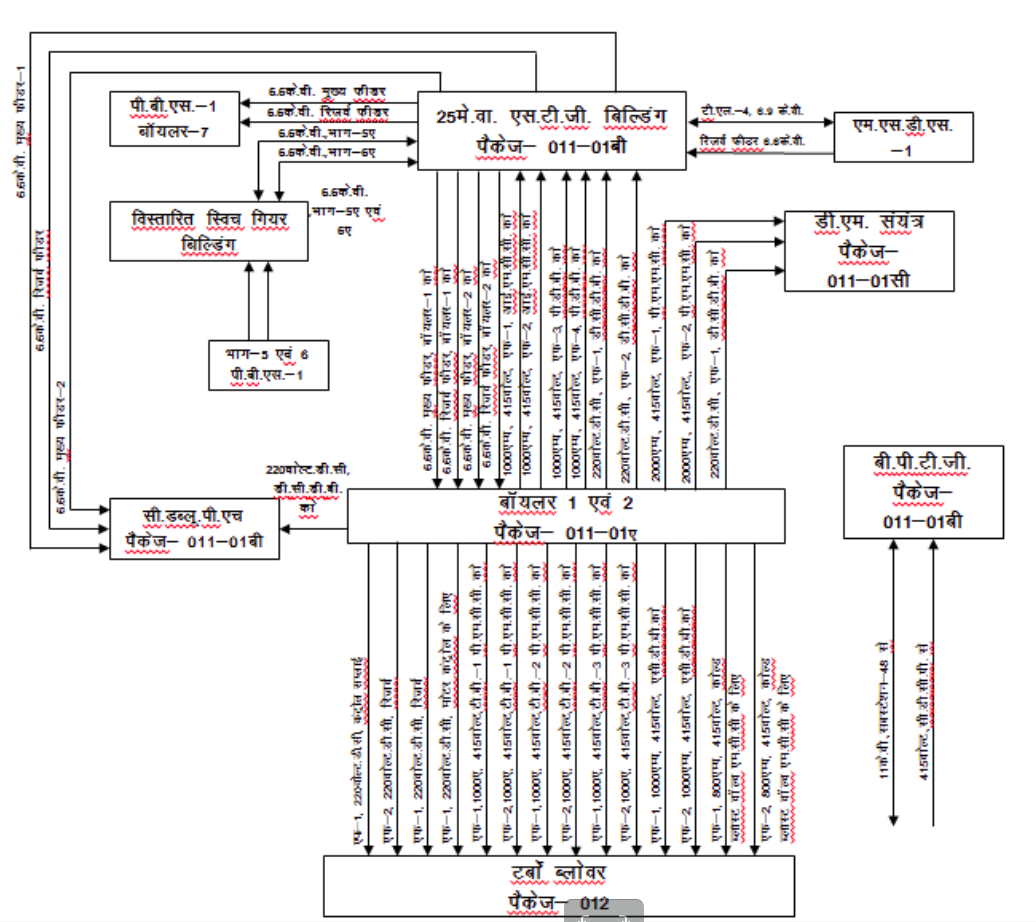
\includegraphics[width = 5in]{sldpbs2.png}
\section{Overview of PBS-2 Electrical Components}
\begin{enumerate}
\item 
Two complete generator sets and their auxiliaries consisting of the following major equipment/systems for the new units.
\begin{itemize}
    \item Generator sets.
    \item Equipment/systems/mechanisms to meet pollution norms like noise
  level, vibration level, etc.
    \item Generator cooling systems.
    \item Generator lubricating oil systems.
    \item Complete excitation systems (brushless type), latest digital AVR
  (thyristor controlled with dual channels and associated electrical
  equipment having data interface with DDCMIS).
    \item Generator line side terminal cubicles consisting of Surge Arrestors, PT,
  CT, Capacitor, Link etc.
    \item Generator neutral cubicles with neutral side CTs.
    \item IG-541 extinguishing and automatic injection system for the
  Generators.
    \item Any other equipment/systems required for smooth running of generator
  sets.
\end{itemize}

\item Transformer - \begin{itemize}
    \item One Generator Transformer of rating 36 MVA, 11/6.9kV, ONAN
        type.
    \item Auxiliary Transformers of rating 2 MVA or 1 MVA, 6.6/0.433 kV, AN
        type.
\end{itemize}

\item Two \textbf{Interconnections} between MSDS-I and PBS-IIa
\begin{itemize}
 \item Tie-line-4- Interconnector between MSDS-I (Sec-IV-Cubicle 36) and PBS-11 sections VII & VIII.
 \item Reserve supply from MSDS-I (Sec-IV cubicle 66) to the Reserve
        6.6kV board at PBS-11.
\end{itemize}
\item Contractor shall provide one set of Generator Control Desk each with respective MIMICs for controlling all the synchronizing breakers detailed as below:
\begin{itemize}
    \item For the 6.9kV switchboard(MSG) Breakers:
       \begin{itemize}
        \item[-]2nos. 6.9kV Generator Breakers of TG-4 connected to Section VII & section VIII
        \item[-]2 Tie-line-4 feeder breakers of Section VII & VIII
        \item[-]2 Sectionaliser breakers connected to Section VII
        \item[-]1  breaker of Section VI(extended) connected to Section VII
        \item[-]2 bus coupler breakers between sections VII & VIII and
           Extended Sections V & VI
        \item[-]2  Inter-connector breakers connected to extended sections of
          Section-V & VI located at PBS-11
        \item[-]2 breakers connected to the existing Sections V & VI located
           at the extended switchgear building at PBS-1
       \end{itemize}
    The above Generator control desks shall be placed at PBS-II premises
    \item For the 11 kV switchboard at BPTG premises
    \begin{itemize}
        \item[-]One no. 11 kV Generator Breaker of BPTG connected to the 11 kV Board
        \item[-]One no. Tie-line feeder breaker of the 11kV switchboard
           connected to the 11 kV switchboard at CDCP area
    \end{itemize}
    The above Generator control desks shall be placed at BPTG premises.
\end{itemize}
\item  Relay and Protection Panel for the Generating units, namely
\begin{itemize}
    \item[-]1 x 25 MW STG
    \item[-]1 x 4 MW BPTG
\end{itemize}
\item 6.9kV Switch Boards(sections VII &VIII, Extended sections V & VI, connecting busduct) including the corresponding reactors, busducts and the isolators.
HT busduct shall be provided for 3150A busduct between Generator Transformer and MSG and 2000A busduct for the
\begin{itemize}
    \item[-]Incoming Tieline-4
    \item[-]Bus coupler between sections VII & VIII and
    \item[-]Bus coupler between sections (extended)sections V & VI
    \item[-]Two interconnectors between sections VII & V
\end{itemize}
\item 11 kV Switch Board at the BPTG station.
\item  6.6kV Switch Board at the CWPH area.
\item 415V Power cum Motor Control Centers (PMCCs) for CWPH and BPTG areas.
\item 415V Motor Control Center for the Steam Turbo Generator.
\item 415V Motor Control Center for the BPTG.
\item 415V Motor Control Center for the Cooling Water system.
\item 415V Motor Control Centers for the AC and Ventilation system.
\item 415V Power Distribution Boards.
\item Electrical Auxiliary Control Panel(EACP) for Remote Control, metering & annunciation panel for the centralized control, metering and annunciation for all the 11 kV, 6.9kV, 6.6 kV and 415V incomers & bus-coupler feeders excluding the feeders mentioned in S.no. 4 above. Separate EACP panels shall be considered for PBS-II
\item Hooking up for control, monitoring and protection of generators and power distribution equipment/systems with DDCMIS. Transducer panels for inputs/outputs from/to electrical equipment to/from DDCMIS. This shall be considered for all the generating sets and its auxiliaries.
\item A dedicated and separate SCADA system shall be provided for Electrical system of PBS II in the Main Control room of the Switchgear Building. The electrical parameters shall be hooked up in this SCADA system for metering , alarm, annunciation and control. The major systems to be covered in the SCADA are as follows:
\begin{itemize}
    \item[-]All HT Breaker Status(ON/OFF/TRIP/Ready to Start) and all
       metering parameters.
    \item[-]All the LT switch gear in PMCC, MCC (I/c & B/c), all DBs (I/c & B/c) and all metering
       parameters. 
    \item[-]All intelligent controllers in MCCs.
    \item[-]Generator protection and metering parameters.
    \item[-]All kinds of Transformer alarm, annunciation and protection.
    \item[-]All kinds of alarm and annunciation for batteries, charger and
      UPS
    \item[-]All the MFMs.
    \item[-]Fault annunciation from all the communication type protective
       relays, meters. From this SCADA, all the relay parameters shall
       be monitored as well as their settings can be changed/configured.
\end{itemize}
\item The new SCADA System shall be hooked up with
\begin{itemize}
     \item[-] The upcoming SCADA for PBS-11 Boiler pkg-011-A.
 \item[-] Existing SCADA system (presently used for existing electrical system
          for Switch gear and generators).
 \item[-] TRT Generator relays (IEC 61850 compliant) located at the TRT
          building for hooking up all the parameters of TRT Generator at PBS-II.
 \item[-] Provision shall also be made for hooking up the entire HT substation
          with the upcoming centralized SCADA system as well as a separate
          gateway shall be provided in the relay for interfacing with the
          instrument SCADA of PBS-11, PBS-I & BPTG Station.
\end{itemize}
SCADA/PLC interfacing shall be as per TS and all networking equipment
required for the completeness of the integration of the proposed SCADA
with the above systems shall be in the scope of the Contractor.
Separate printers (Laser) shall be provided for both the stations.
Wherever signal is to be duplicated for hooking upto two different systems
(DDCMIS & SCADA) Signal Multiplier (Optical/Galvanic Isolator) may be
considered.
Furniture required to mount work station for SCADA including provision for
operator chairs on the basis of one for each station in the new electrical            control room of PBS-II (Six chairs &six tables with sufficient drawers for storing    documents for MMIs and generator protection Terminal)
\item he entire Contractor's equipment at BPTG station shall be hooked up
with their BPTG station PLC/DCS as well as to the PLC / DCS at power
and blowing station for complete control, monitoring, sequencing,
metering and protections monitoring including alarm and annunciations.
The Contractor in all their equipment at BPTG station shall make the
necessary arrangement for the same. All cabling including terminations at
both ends are included in the scope of the Contractor.
\item  Two DCDBs for generator control and protection as well as for
HT/LT substation requirement for PBS-2 & CWPH areas. These DCDBs
shall be fed from the DC system of Boiler Pkg-01A. Necessary cabling
from the Employer's switchboard to the DCDB shall be considered in the
scope of the Contractor.

\item One set DC System including battery, charger, DCDB, etc for BPTG
station.

\item PDBs- Power supply to UPS, Battery chargers, illumination, etc shall be
fed from PDB. A separate PDB shall be provided for crane, welding
sockets, etc.

\item UPS system complete in all respects individually one set each for TG
building, BPTG System and Cooling water control system.

\item UPS Distribution boards.

\item HT & LT motors including DC motors and actuators.

\item Motorized control/isolation valves with manual operating handles.

\item HT & LT power and control cabling including their termination at both
      ends and jointing/termination materials.

\item Signal and instrumentation cables, special cables, screened cables, fire
optic cables, etc including their termination at both ends (supply as well
as laying & termination shall be under Contractor's scope).

\item Cable trestle, supporting structures, conduits, prefabricated GI cable
trays, cable racks, other associated accessories like cable glands, lugs,
termination/jointing kits, ferrules, clamps including trefoil clamps for single
core cables, cable markers, cable identification tags, and all other
hardware material as per requirement.

\item Supply, laying of cables and termination at both the ends of all
interconnecting power, control, signaling and instrumentation cables etc
between Contractor's own equipment and between Contractor's
equipment and Employer's equipment for all incoming power supplies etc.
to make their system complete in all respect along with others 
\item Local Push button stations.

\item Islanding and load shedding system shall be provided for grid islanding
due to grid disturbances and load shedding shall be planned due to
unbalanced of load requirement and generation during generator in
islanding mode. Philosophy for the same shall be finalized during detail
engineering.

\item Welding sockets, Power receptacles, etc.

\item Monorail arrangement for handling Transformers in Transformer Rooms.

\item Monorail for HT/LT motors and canopy over outdoor HT/LT motors.

\item Complete illumination of Power and Blowing station-TG building,
extended Switchgear building, CWPH area and BPTG plant, Plant road
and area illumination,etc and all other areas within limit with sufficient
numbers of LDBs /SLDBs.
Lighting fixtures of electrical rooms shall be industrial, energy
efficient fluorescent type with electronic chokes. Control room shall
have energy efficient CFL type lamps.
\item All erection materials, required during erection of generator and
auxiliaries and all types of electrical equipment under Contractor's scope.

\item DC starter panels for DC motors.

\item HT Soft starters.

\item Complete electrics of material handling equipment like cranes, lifts,
hoists, etc.

\item Complete electrics of air-conditioning and ventilation systems in all the
premises under battery limit.

\item Water drainage pumps in required numbers with complete electrics
including source feeders , pumps/motors, cable laying, etc.


\item Fire protection system including Fire Detection and Alarm System for the
complete plant, etc.

\item One unit each of Thermo-vision camera , DC earth fault locator- Model
Grouser fault finder, 300V DC.

\item Safety items.
\item Training courses for the Employer's personnel/Engineers to acquire
necessary expertise in operation and maintenance of the Plant &
Equipment of the electrical system for atleast for 120 mandays at works.

\item Complete relay coordination including relay setting calculations for all
relays for complete Generation and Power Distribution system at various voltage levels (415V, 6.9kV, 6.6 kV, 11 kV) are under the scope of the Contractor. Necessary system study if required to be conducted by the Contractor.\\
\newpage
\subsection{Standard Voltage Levels}
Following power utilization standard voltage levels shall be adopted for various systems\\
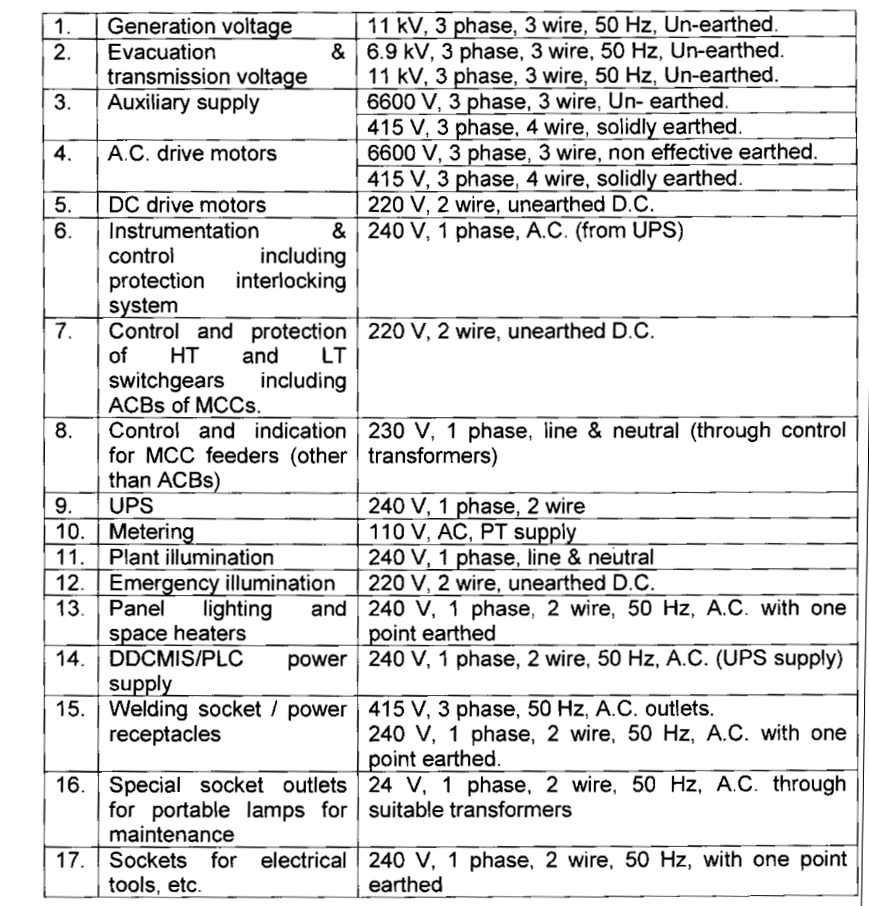
\includegraphics[width = 6in]{stanvoltlevel.png}
\subsection{Rating}
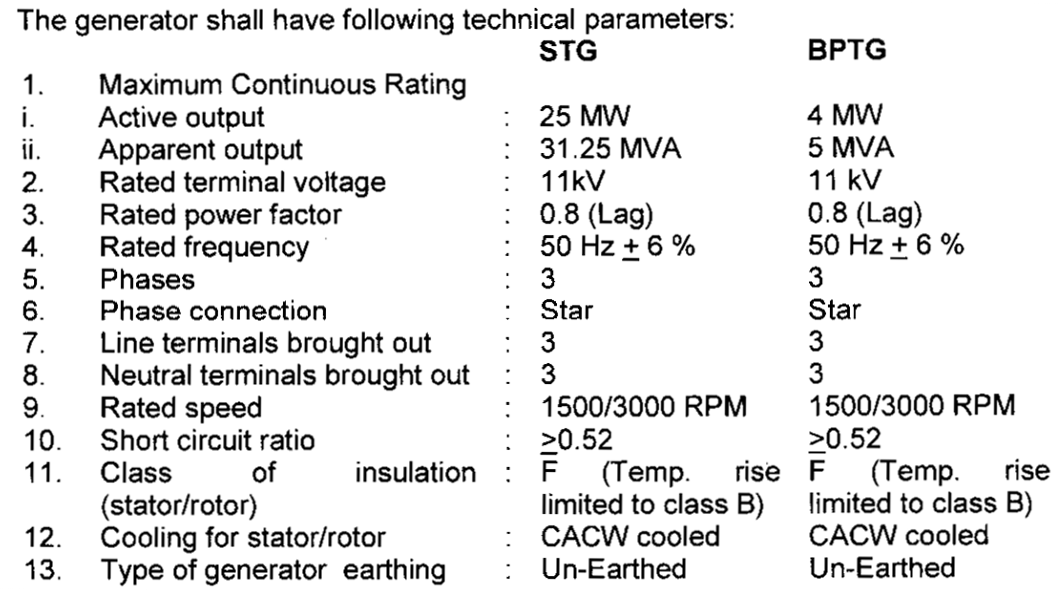
\includegraphics[width = 6in]{rating.png}


\end{enumerate}




\chapter{D.M. Water Plant}
Raw water from reservoirs at \textbf{Maroda} is required to be treated before it can be used in boilers. The process of softening raw water is shown below.\\
\begin{center}
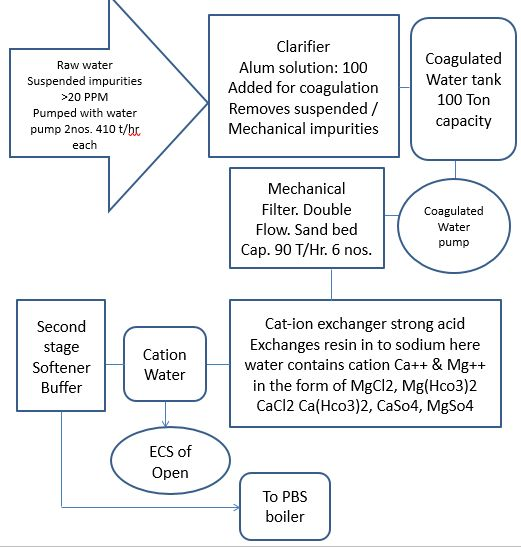
\includegraphics[width = 4.2in]{dmprocess.png}\\
\end{center}

$$\ce{R(Resin) + Na2 + Ca -> CaR + 2NaHCO3}$$
$$\ce{R(Resin) + Na2 + CaCl2 -> CaR + 2NaCl}$$
Regeneration is done back to get back Na ions.
\section{Introduction}
\textbf{Demineralization} is the process of removing mineral salts from Water by using the ion exchange process.
Demineralised Water is Water completely free (or almost) of dissolved minerals as a result of one of the following processes:
\begin{itemize}
    \item Distillation
    \item Deionization
    \item Membrane filtration (reverse osmosis or nanofiltration)
    \item Electrodyalisis
    \item Or other technologies.
\end{itemize}
Demineralized Water also known as Deionized Water, Water that has had its mineral ions removed. Mineral ions such as cations of sodium, calcium, iron, copper, etc and anions such as chloride, sulphate, nitrate, etc are common ions present in Water. Deionization is a physical process which uses specially-manufactured ion exchange resins which provides ion exchange site for the replacement of the mineral salts in Water with Water forming H+ and OH- ions. Because the majority of Water impurities are dissolved salts, deionization produces a high purity Water that is generally similar to distilled Water, and this process is quick and without scale buildup. De-mineralization technology is the proven process for treatment of Water. A DM Water System produces mineral free Water by operating on the principles of ion exchange, Degasification, and polishing. Demineralized Water System finds wide application in the field of steam, power, process, and cooling.

\section{Principle}
Raw Water is passed via two small polystyrene bead filled (ion exchange resins) beds. While the cations get exchanged with hydrogen ions in first bed, the anions are exchanged with hydroxyl ions, in the second one.

\section{Process}
In the context of Water purification, ion-exchange is a rapid and reversible process in which impurity ions present in the Water are replaced by ions released by an ion-exchange resin. The impurity ions are taken up by the resin, which must be periodically regenerated to restore it to the original ionic form. (An ion is an atom or group of atoms with an electric charge. Positively-charged ions are called cations and are usually metals; negatively-charged ions are called anions and are usually non-metals).\\
The following ions are widely found in raw waters : \\
\textbf{Cations}-
\begin{itemize}
    \item Calcium (Ca2+)
    \item Magnesium (Mg2+)
    \item Sodium (Na+)
    \item Potassium (K+)
\end{itemize}
\textbf{Anions}-
\begin{itemize}
    \item Chloride ( Cl-)
    \item Bicarbonate (HCO3-)
    \item Nitrate (NO3-)
    \item Carbonate (CO32-)
\end{itemize}

\section{Ion Exchange Resins}
There are two basic types of resin - cation-exchange and anion-exchange resins. Cation exchange resins will release Hydrogen (H+) ions or other positively charged ions in exchange for impurity cations present in the Water. Anion exchange resins will release hydroxyl (OH-) ions or other negatively charged ions in exchange for impurity anions present in the Water.\\
The application of ion-exchange to Water treatment and purification. \\
There are \textbf{three ways} in which ion-exchange technology can be used in Water treatment and purification :
\begin{itemize}
    \item cation-exchange resins alone can be employed to soften Water by base exchange
    \item anion-exchange resins alone can be used for organic scavenging or nitrate removal
    \item ombinations of cation-exchange and anion-exchange resins can be used to remove virtually all the ionic impurities present in the feedWater, a process known as \textbf{deionization}. Water deionizers purification process results in Water of exceptionally high quality
\end{itemize}

\section{Deionization}
For many laboratory and industrial applications, high-purity Water which is essentially free from ionic contaminants is required. Water of this quality can be produced by deionization.The two most common types of deionization are :
\begin{itemize}
    \item Two-bed deionization
    \item Mixed-bed deionization
\end{itemize}
\subsection{Two-bed deionization}
The two-bed deionizer consists of two vessels - one containing a cation-exchange resin in the hydrogen (H+) form and the other containing an anion resin in the hydroxyl (OH-) form. Water flows through the cation column, whereupon all the cations are exchanged for hydrogen ions. To keep the Water electrically balanced, for every monovalent cation, e.g. Na+, one hydrogen ion is exchanged and for every divalent cation, e.g. Ca2+, or Mg2+, two hydrogen ions are exchanged. The same principle applies when considering anion-exchange. The decationised Water then flows through the anion column. This time, all the negatively charged ions are exchanged for hydroxide ions which then combine with the hydrogen ions to form Water (H2O).

\subsection{Mixed-bed deionization}
In mixed-bed deionizers the cation-exchange and anion-exchange resins are intimately mixed and contained in a single pressure vessel. The thorough mixture of cation-exchangers and anion-exchangers in a single column makes a mixed-bed deionizer equivalent to a lengthy series of two-bed plants. As a result, the Water quality obtained from a mixed-bed deionizer is appreciably higher than that produced by a two-bed plant. Although more efficient in purifying the incoming feedWater, mixed-bed plants are more sensitive to impurities in the Water supply and involve a more complicated regeneration process. Mixed-bed deionizers are normally used to ‘polish' the Water to higher levels of purity after it has been initially treated by either a two-bed deionizer or a reverse osmosis unit.
\section{Electrodeionization EDI}
Electrodeionization Systems remove ions from aqueous streams, typically in conjunction with reverse osmosis (RO) and other purification devices. Our high-quality deionization modules continually produce ultrapure Water up to 18.2MW/cm. EDI may be run continuously or intermittently.
\section{Advantages of DM Water Plant}
\begin{itemize}
    \item Variety of cost effective standard models.
    \item Improved aesthetics and rugged design.
    \item User friendly, low maintenance and easy to install.
    \item Simpler distribution and collection systems.
    \item Quick availability.
    \item Pre dispatch assembly check.
    \item The multiport valves are top mounted as well as side mounted with the necessary high pressure rating PVC piping.
    \item Single valve operation as compared to the six valves in conventional filters
    \item Each operating step is clearly marked on the valve, thereby eliminating chances of error in the operating sequence.
    \item Single valve assembly, with its simplified frontal Piping, simpler distribution collecting systems is Very easy to install.
    \item Rust free
    \item Less power consumption
    \item Durable
    \item Economical
    \item High shelf life
\end{itemize}
\section{Process Flow Chart}
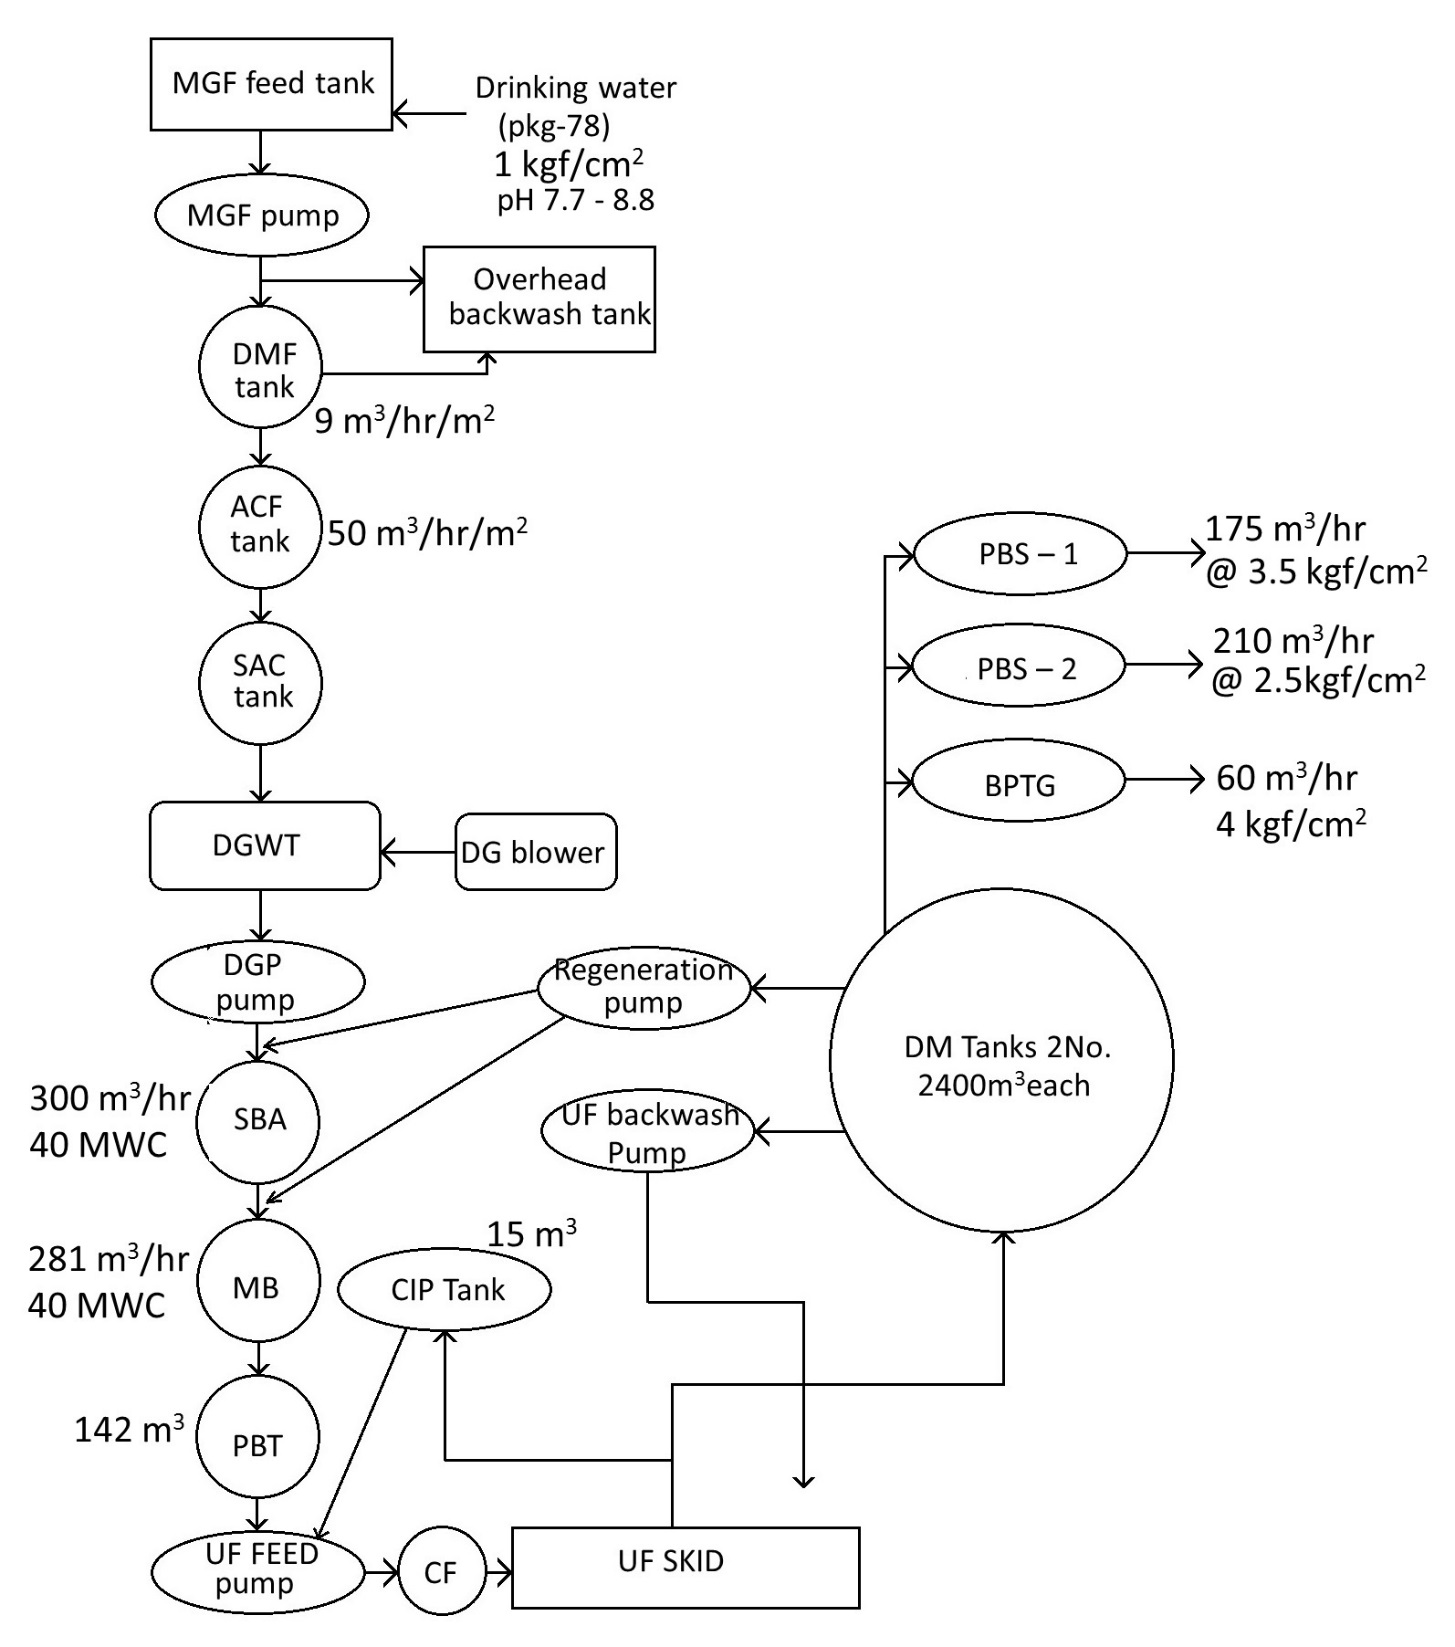
\includegraphics[width = 5in]{dmprocess.jpg}
\section{Plant capacity}
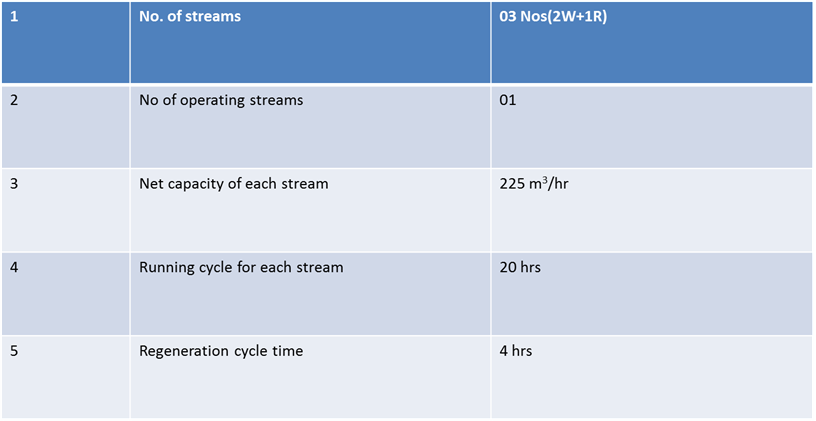
\includegraphics[width = 6in]{dm1.png}
\section{Average water quality report of Maroda-2}
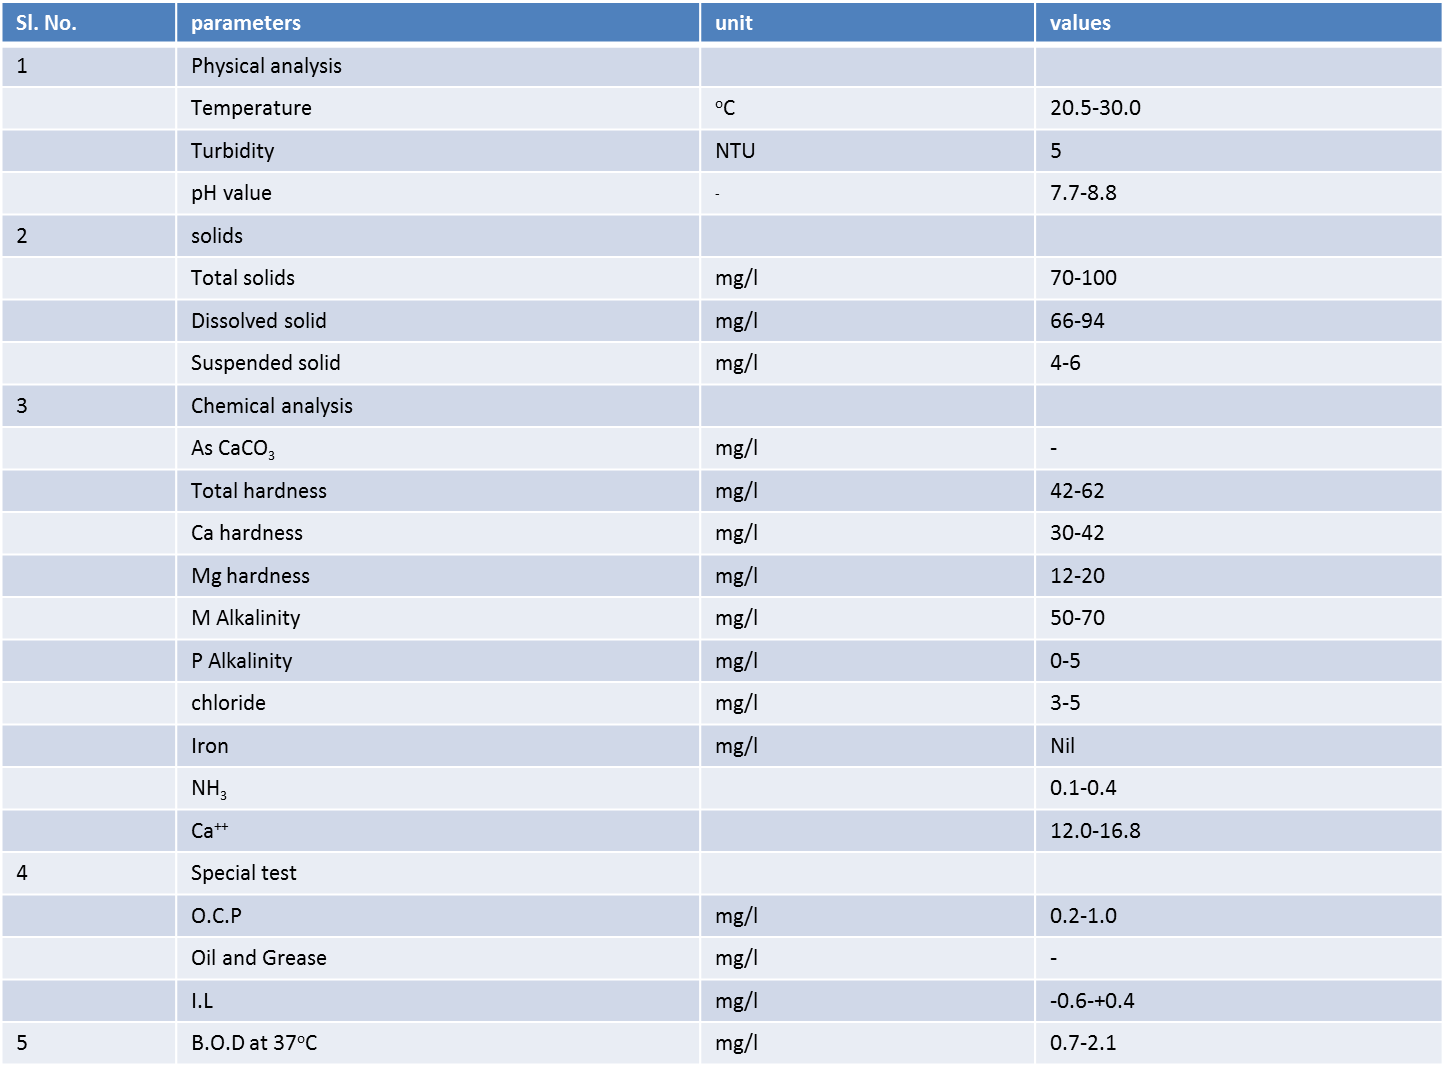
\includegraphics[width = 6in]{dm2.png}
\section{Stage wise treated water quality}
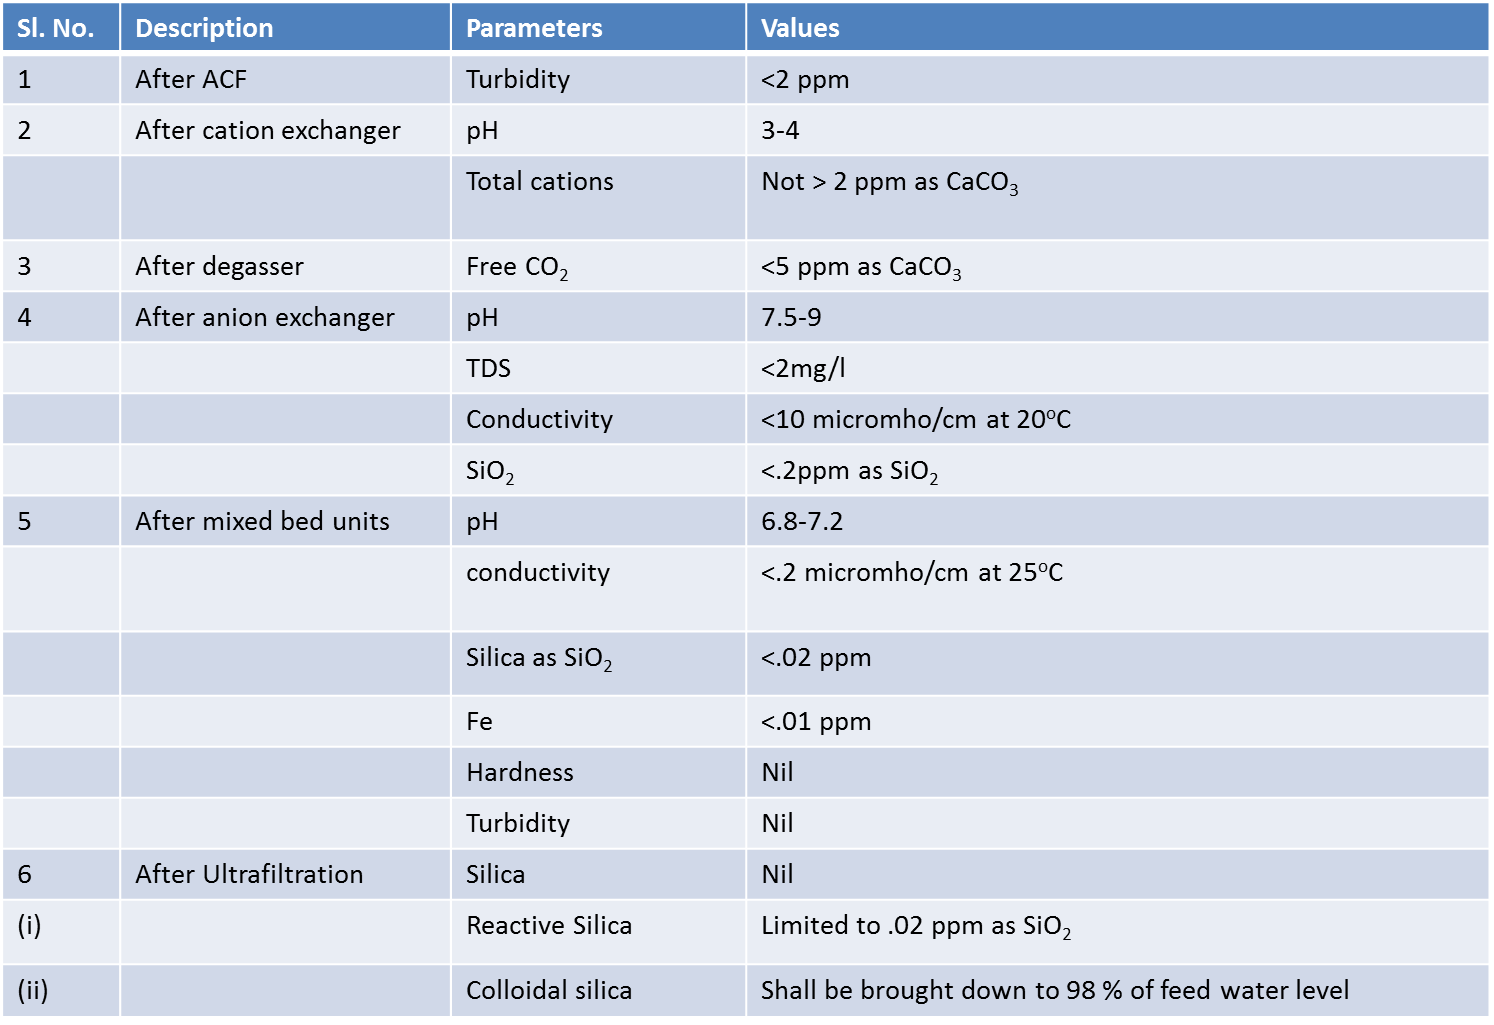
\includegraphics[width = 6in]{dm3.png}
\section{Regeneration flows for SAC}
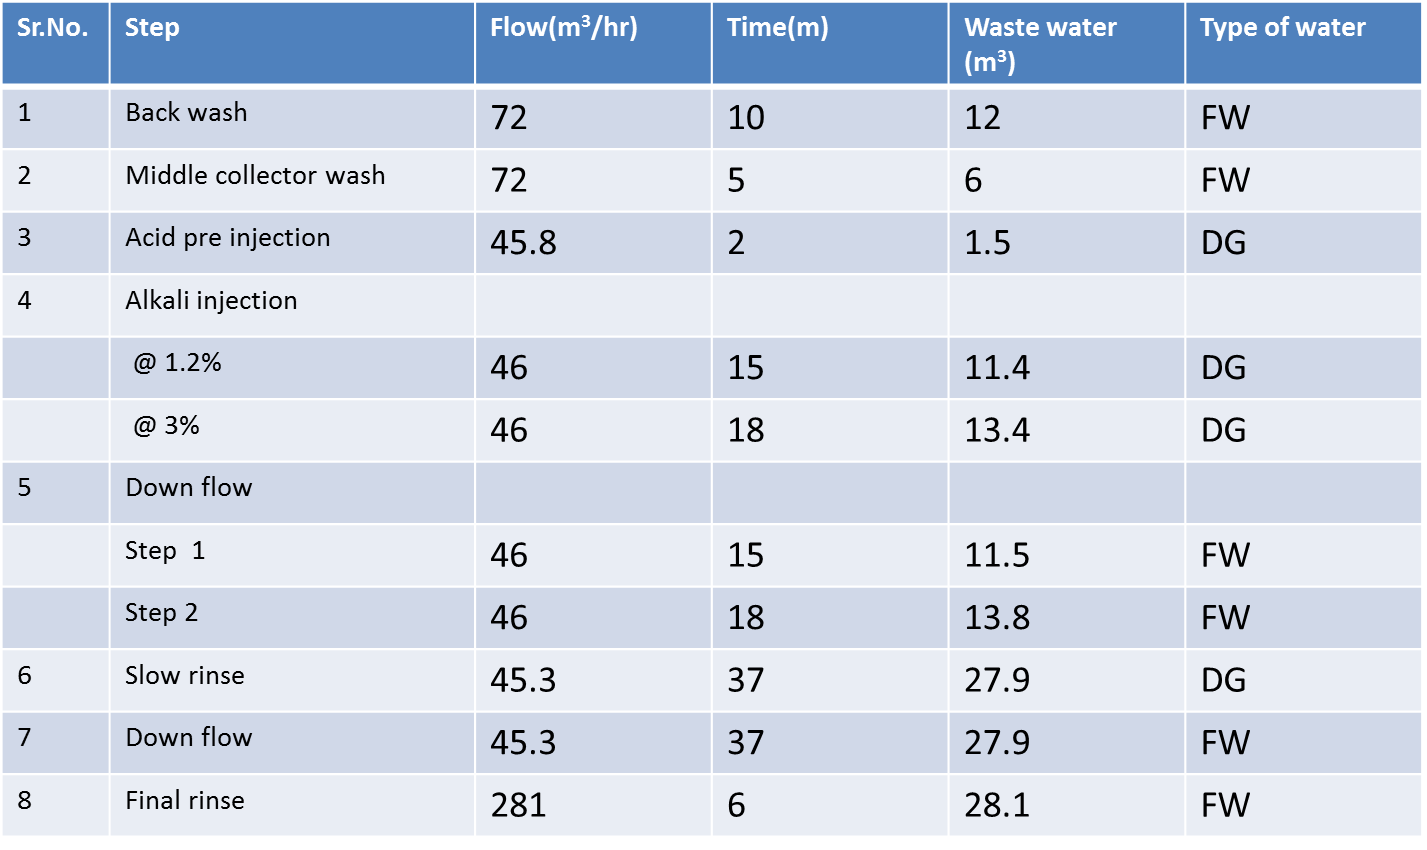
\includegraphics[width = 6in]{dm4.png}
\section{Regeneration flows for SBA}
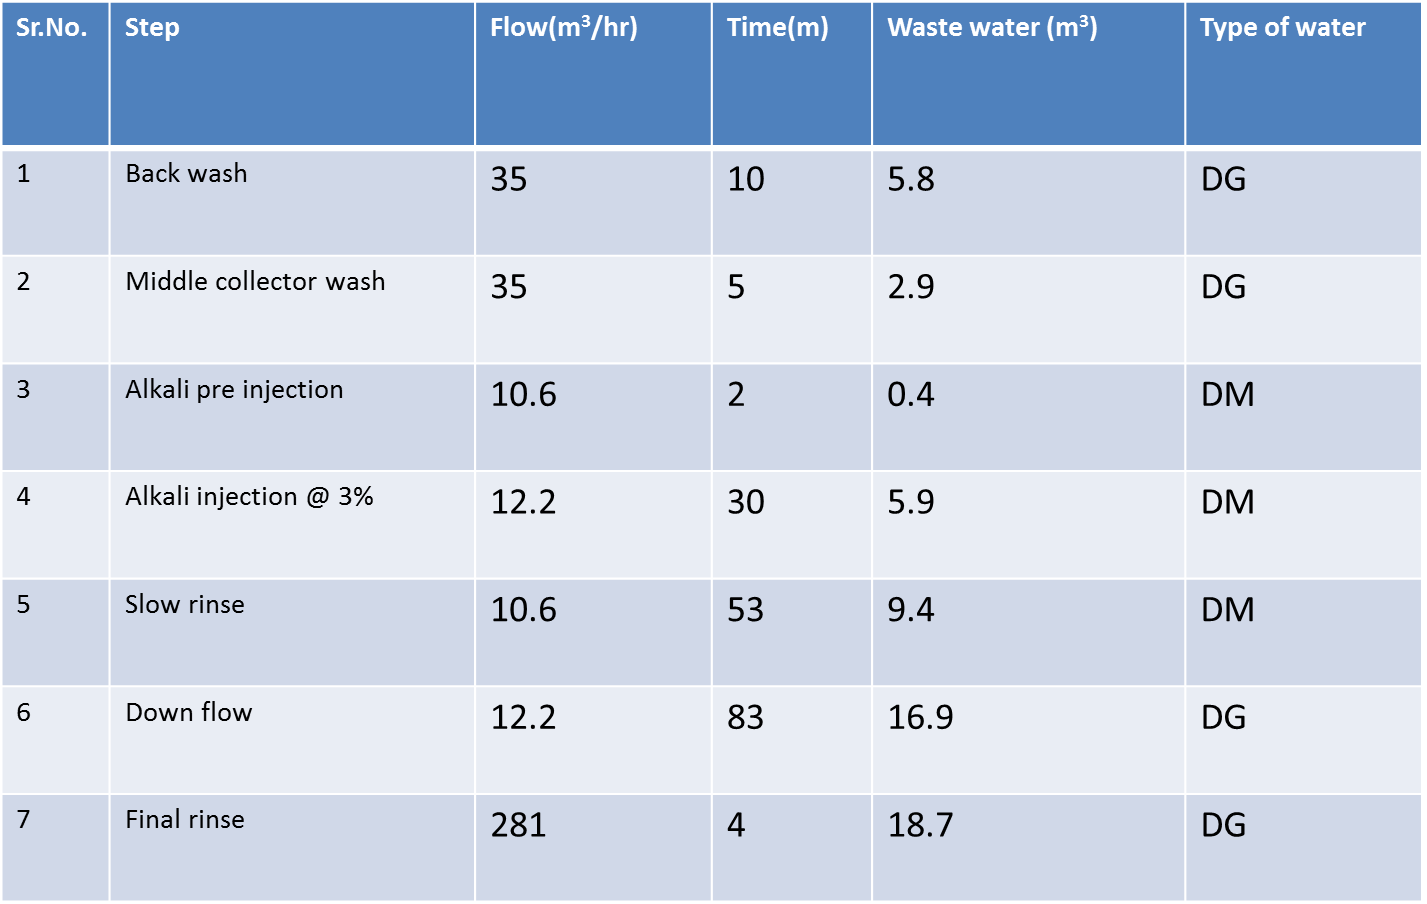
\includegraphics[width = 6in]{dm5.png}
\section{Regeneration flows for mixed bed}
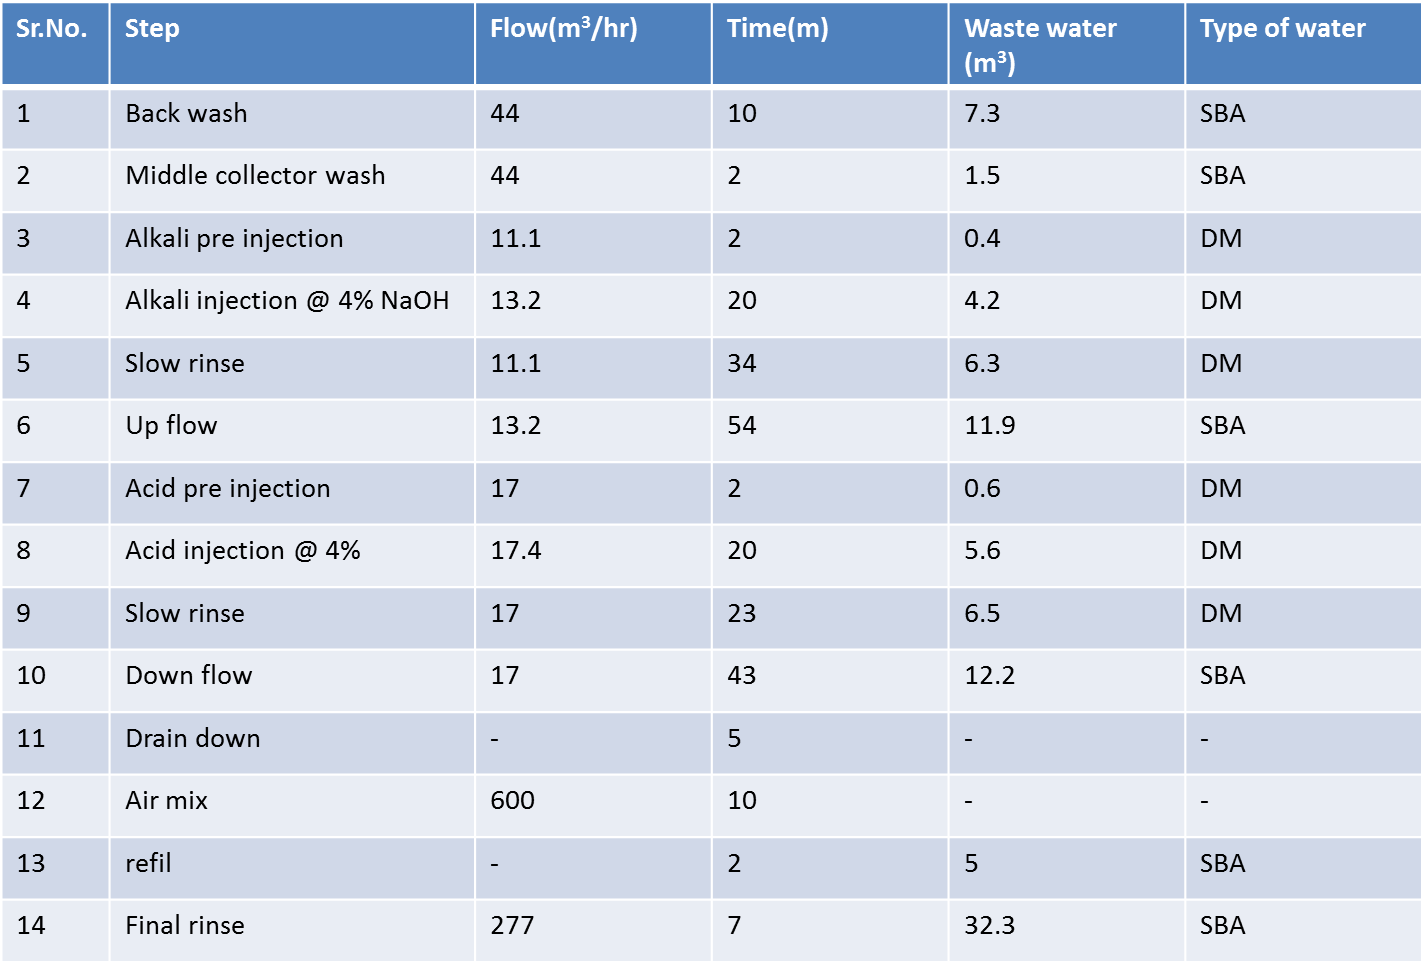
\includegraphics[width = 6in]{dm6.png}
\section{Master Equipments List}
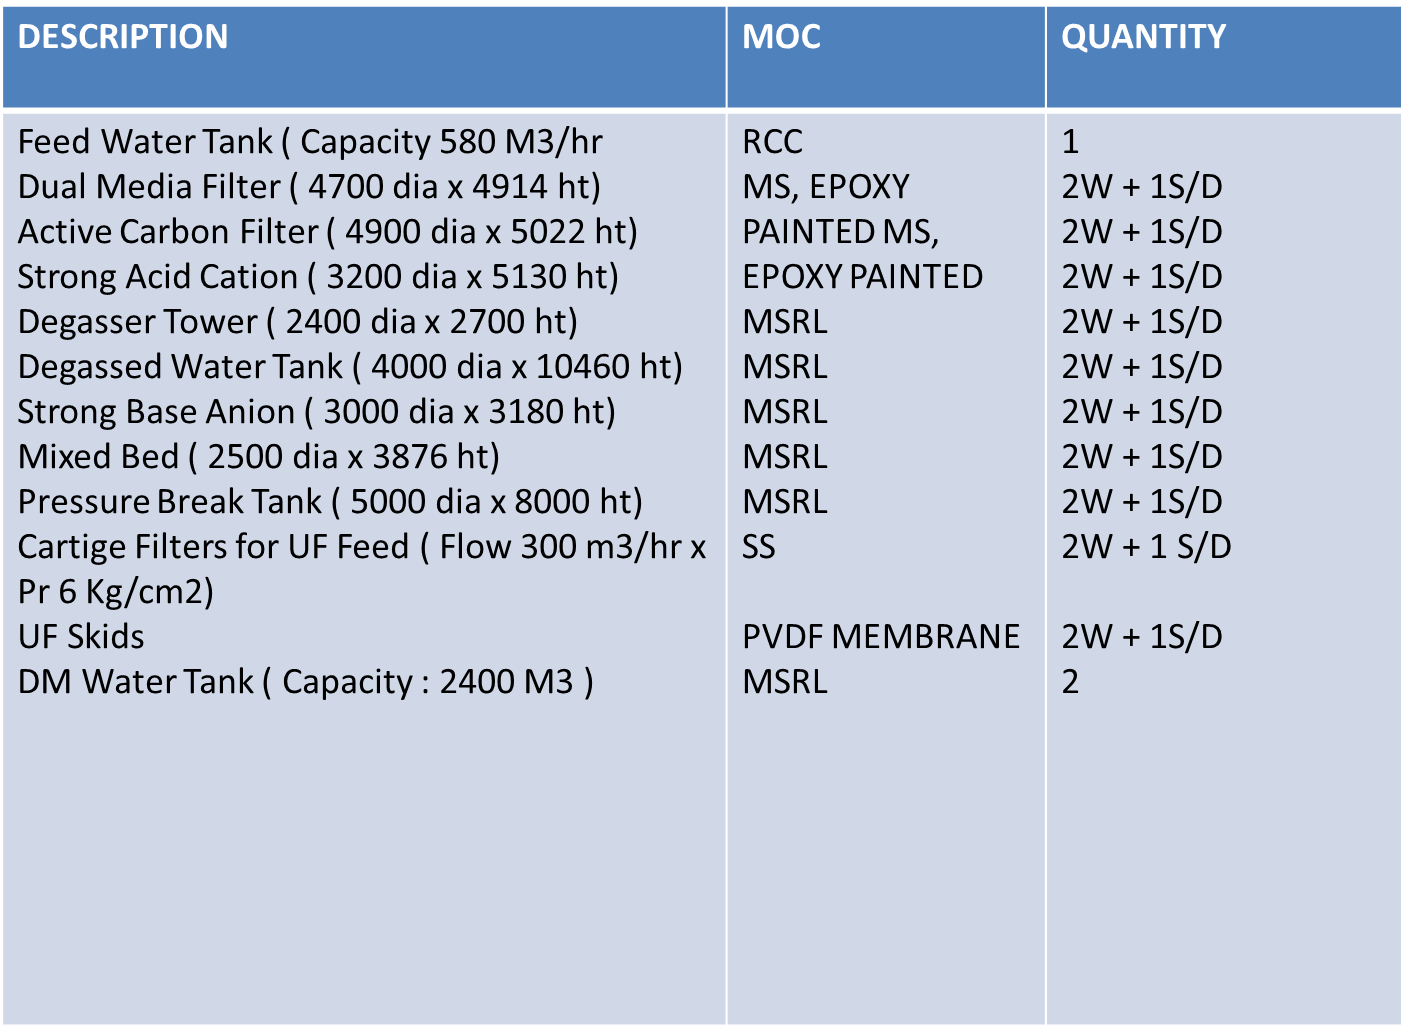
\includegraphics[width = 6in]{dm7.png}
\section{D.M. Water Plant Load Calculations}
\begin{center}
\begin{tabular}{|c|c|}
    \hline
    Raw Water Pump & 2 X 75 = 150 kW \\ \hline
    Transfer Pumps & 30 + 45 + 70 = 145kW \\ \hline
    Degasser Pump & 2 X 55 = 110 kW \\ \hline
    UF Pump & 2 X 45 = 90 kW \\ \hline
    DG Blower & 2 X 3.7 = 7.4 kW \\ \hline
    Regeneration Load & 150 kW \\ \hline
    Aux. Load & 80 kW \\ \hline
    Total Rated load & 737.4 kW \\ \hline
    \textbf{Act. load(80\%) }& \textbf{590 kW} \\ \hline
\end{tabular}
\end{center}

\chapter{Back Pressure Turbo-Generator (BPTG)}
\section{Introduction}
Steam is a major energy user and many industrial processes end up wasting some of it; especially if it is produced at higher pressures than what is needed. The conventional approach is to install pressure-reducing valves (PRVs) at various locations to reduce the steam pressure, exhausting the steam to the atmosphere. However, a non-condensing or backpressure turbine, also called a backpressure turbogenerator, can reduce the pressure while simultaneously converting the exhaust steam into electricity.\\
The steam is expanded until it reaches a pressure that the facility can use. While the steam expands, part of its thermal energy is converted into mechanical energy to be used by pumps, fans, compressors, and other equipment. The steam which has lower pressure  is exhausted into the process header from the steam turbine, where a nozzle directs jets of high-pressure steam against the turbine's rotor blades. These blades are attached to a shaft, which rotates to produce power for the electrical generator. Because the exhaust steam temperature is lower compared with a PRV, the boiler steam throughput must be increased by 5\% to 7\%.\\
A backpressure steam turbine has a power generation efficiency ranging from 15\% to 35\% and requires steam of 20 to 100 lb/h per kilowatt (kW). The turbine operates with an exhaust equal to or in excess of atmospheric pressure. In general, installed cost ranges from \$400/kW to \$800/kW. Not all plants are candidates for backpressure turbines, as the following table shows:\\

% \begin{tabular}{|p{3cm}|p{3cm}|p{3cm}|p{3cm}| }
%  \hline
%  \multicolumn{4}{|c|}{\textbf{\Large{Required Conditions for a Backpressure Steam Turbine}}} \\ [5ex]
%  \hline
%  \textbf{Parameter} & \textbf{Best for Pressure Reducing Valve} & \textbf{Good for Backpressure Turbin}e & \textbf{Best for Backpressure Turbine} \\ \hline
%  Steam Flow Rate (lbm/h) & <4,000 & <4,000  & >10,000  \\ \hline
%  Inlet Pressure (psig) & <125 & >125 & >150 \\ \hline
%  Pressure Drop (psi) & <100 & >100 & >150 \\ \hline
%  Cost of Electricity (cents/kWh) & <1.5 & >1.5 & >6 \\ \hline
%  Capacity Factor (\%) & <25 & >25 & >50 \\ \hline
%  \multicolumn{4}{|c|}{Note: lbm/h=pound mass per hour, psig=pounds per square inch gauge. Source: TurboSteam.} \\[5ex] \hline
% \end{tabular}

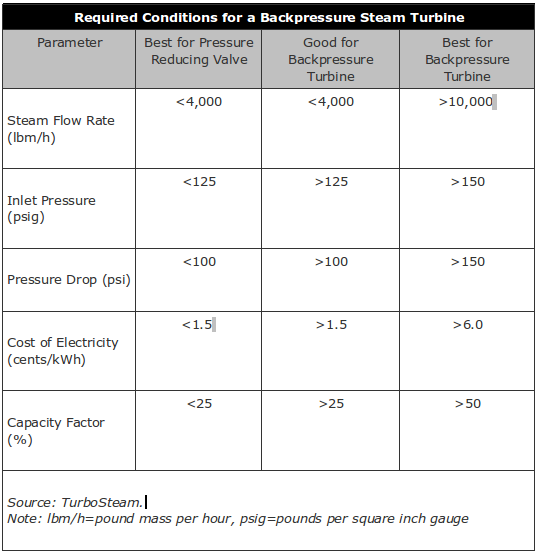
\includegraphics[width = 6in]{dmt1.png}
\\[1em]
Maintenance is minimal for these turbines, as long as both the steam and oil are of good quality. Changing the oil and checking the bearings should be done periodically. Service life is typically 20 years, with some turbines lasting as long as 50 years, when properly maintained. At one chemical plant, a 450-kW system using 110-psi steam operates 24 hours a day, five days per week, with few problems.

\section{Reduce Costs and Lower Emissions}
According to the U.S. Department of Energy (DOE), electricity produced by backpressure turbines can cost less than 3 cents/kWh. Payback can be under two years. After a new clinical research center at the National Institutes of Health installed backpressure turbines, the building generated about 5\% of its own electricity, saving more than \$170,000 annually in electricity costs. When combined with a high-efficiency boiler (80\%), effective electrical efficiencies can reach as high as 78\%. The following table compares the economics of two different systems:\\[1em]
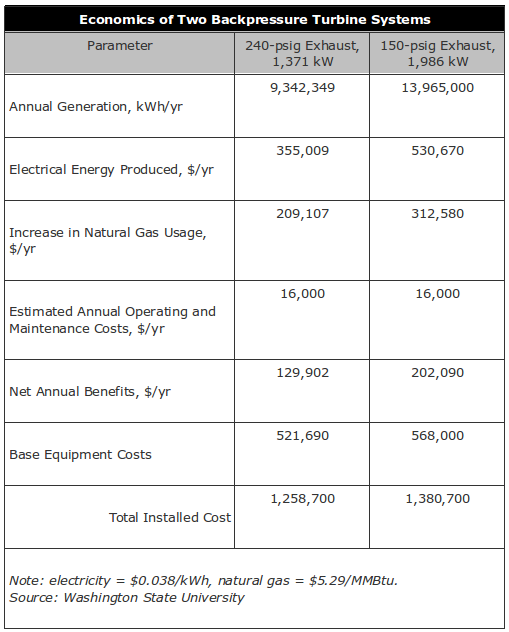
\includegraphics[width = 6in]{dmt2.png}
\\[1em]
Although backpressure steam turbines do not generate any emissions, the steam generator or boiler does. Emissions will depend on the type of boiler fuel, and as shown in the following table, natural gas generates the fewest total emissions:\\[1em]
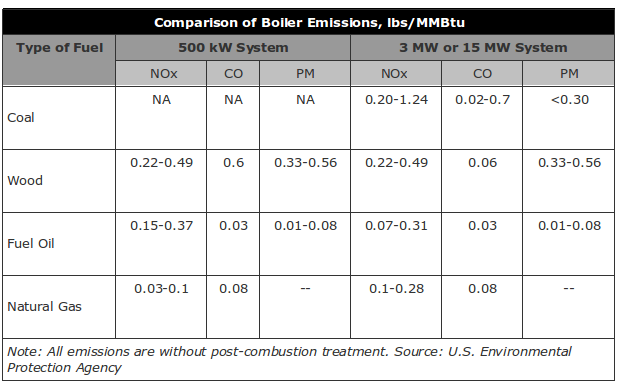
\includegraphics[width = 6in]{dmt3.png}

\section{Flow Diagram of Steam in BPTG}
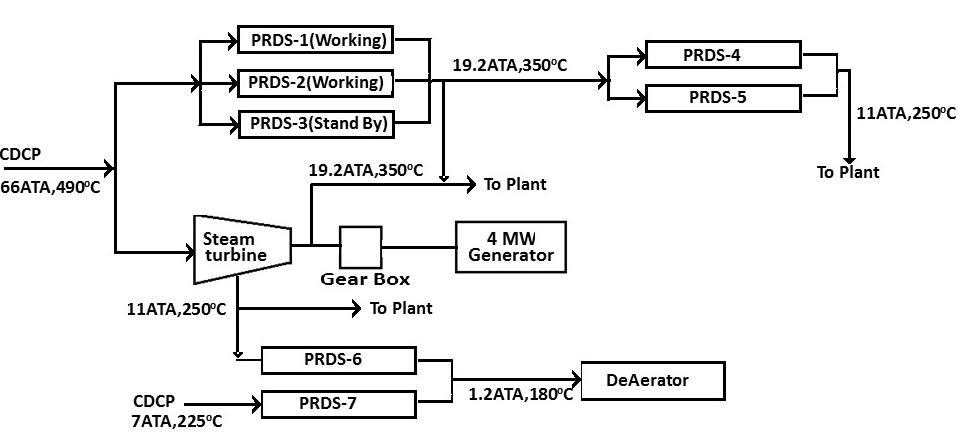
\includegraphics[width = 6in]{bptgflow.png}

\section{Deaerator in BPTG}
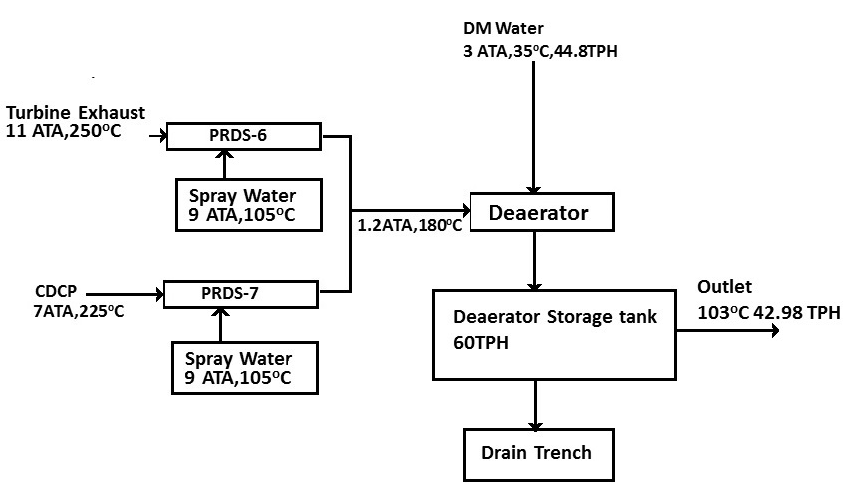
\includegraphics[width = 6in]{bptgdeaerator.png}

\section{BPTG Load Calculations}
\begin{center}
\begin{tabular}{ |c|c|c| } 
 \hline
 Transfer Pump & 30 kW \\ \hline
 Spray Water Pump & 22 kW \\ \hline
 CW Pump & 2 X 30 kW = 60 kW \\ \hline
 CT Fan & 11 kW \\ \hline
 Turbine Pumps & 15 kW \\ \hline
 Aux. load & 250 kW \\ \hline
 Total Rated Load & 388 kW \\ \hline
 \textbf{Act. loa}d & \textbf{310 kW} \\ \hline
\end{tabular}
\end{center}

\chapter{25 MW Steam Turbo Generator (STG)}
\section{Introduction}
A turbo generator is the combination of a turbine directly connected to an electric generator for the generation of electric power. Large steam-powered turbo generators provide the majority of the world's electricity and are also used by steam-powered turbo-electric ships.\\
Smaller turbo-generators with gas turbines are often used as auxiliary power units. For base loads diesel generators are usually preferred, since they offer better fuel efficiency, but, on the other hand, diesel generators have a lower power density and hence, require more space.\\
The efficiency of larger gas turbine plants can be enhanced by using a combined cycle, where the hot exhaust gases are used to generate steam which drives another turbo generator.
\section{Front View}
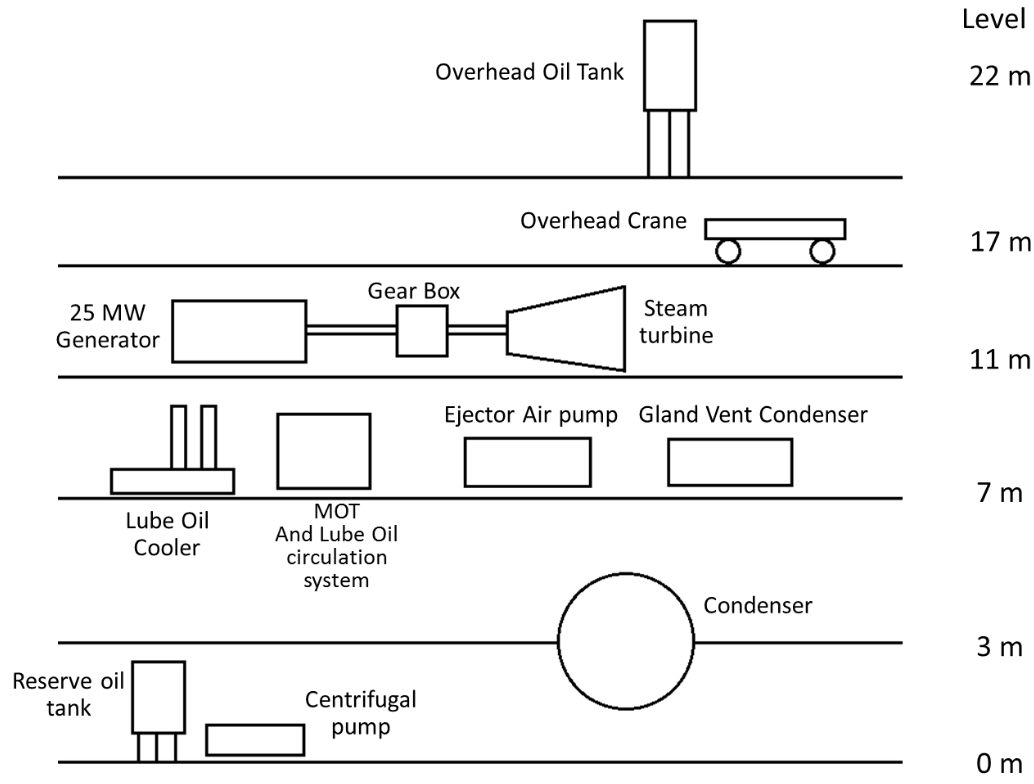
\includegraphics[width = 6in]{stgfront.png}

\section{Process Flow Diagram}
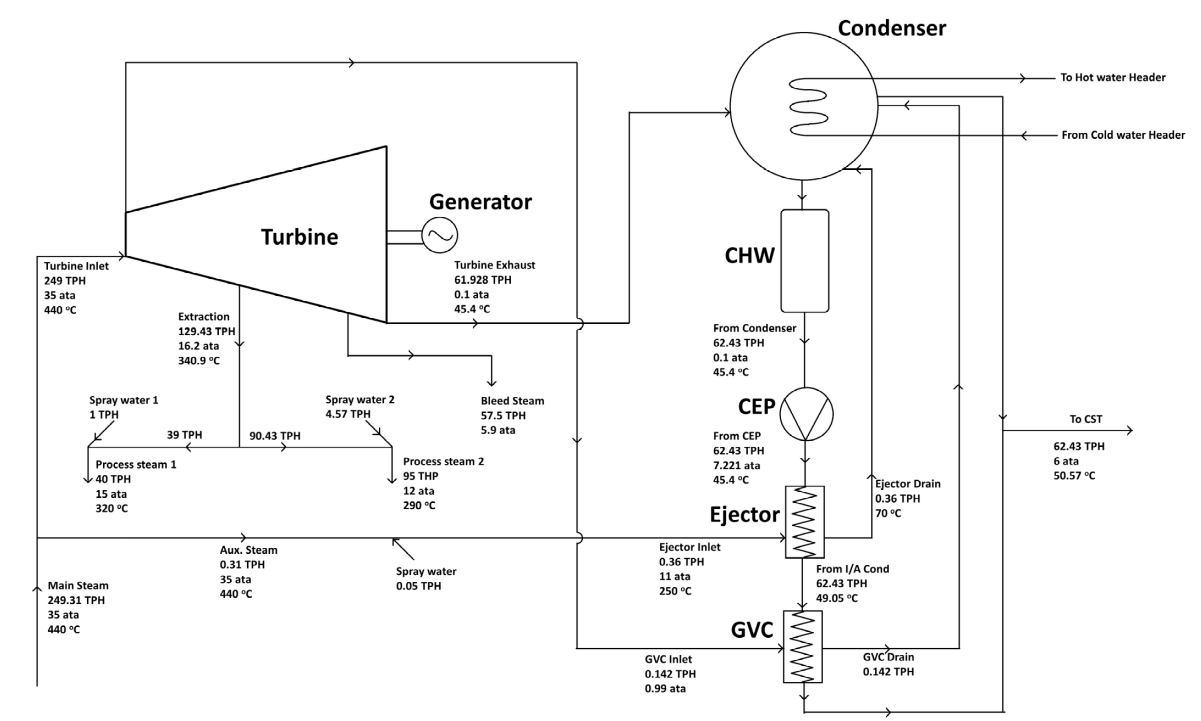
\includegraphics[width =6in]{stgprocessflow.png}

\section{Mechanical Component}
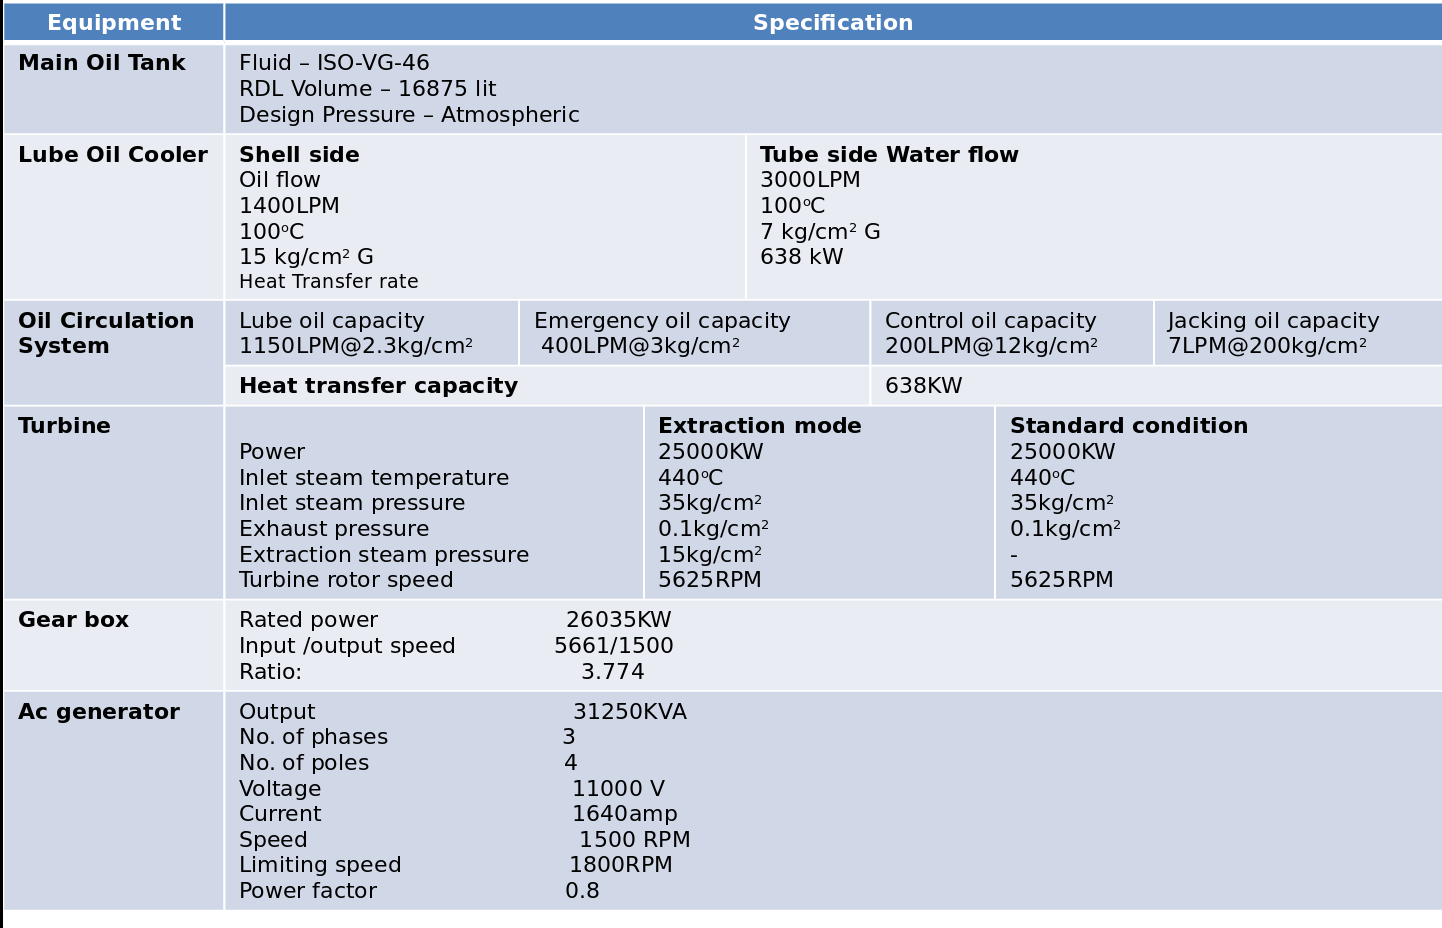
\includegraphics[width =6in]{stgmech.png}

\section{Electrical Component}
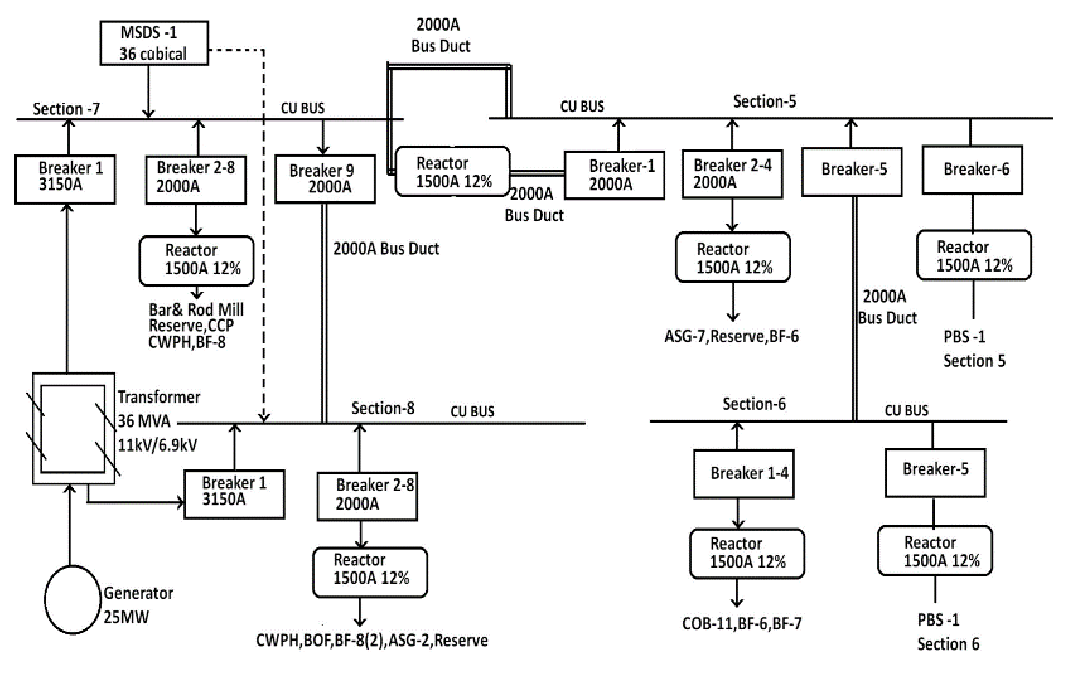
\includegraphics[width =6in]{stg25mw}

\section{Electrical Reserve Supply Switch Board}
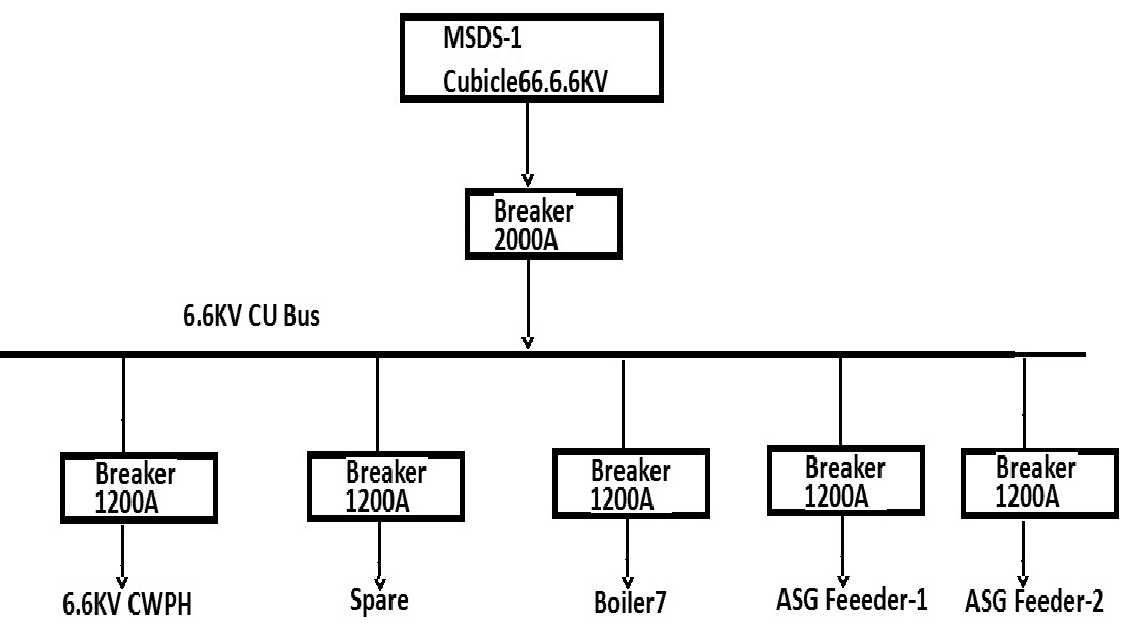
\includegraphics[width =6in]{stgelec} 

\section{Electrical Equipment}
\begin{center}
\begin{tabular} { | c | c | c |} 
\hline
Equipment & Specification & Location \\ \hline
Transformers & 36MVA, 11kV/6.9kV & 0 meters B-C \\ \hline
Breakers & 1.3150 Amp, 2.2000 Amp & 11 meters A-B \\ \hline
Reactor & 1500 Amp, 12\% & 3 meters A-B \\ \hline
DCS &  & 11 meters \\ \hline
LT Panels & & 11 meters\\  
\hline
\end{tabular}
\end{center}  



\section{Technical Data Sheet of Auxiliary Transformer}
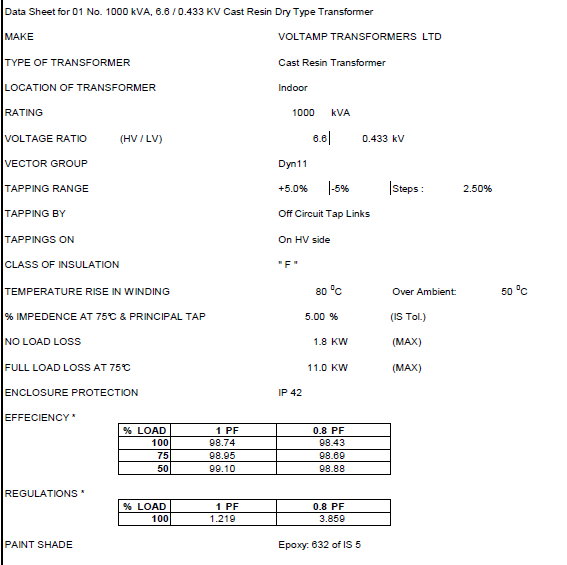
\includegraphics[width =6in]{stgtech1.png} 
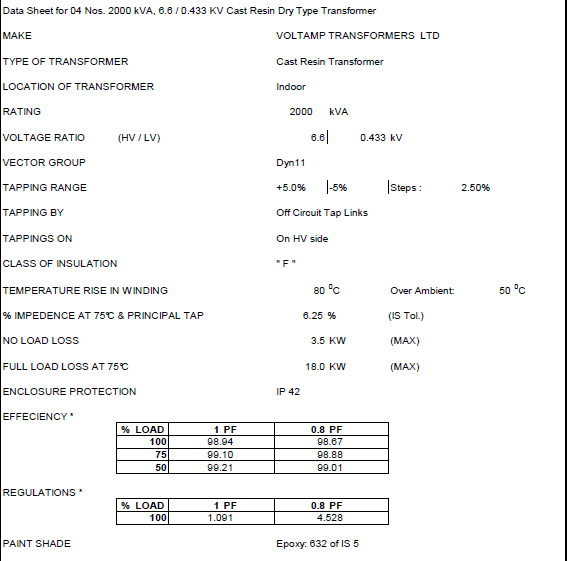
\includegraphics[width =6in]{stgtech2.png} 

\section{Approved 25MW STG, ESGB & RSSB SLD}
Click \href{http://i.imgur.com/8oG8HFV.jpg}{here} for detailed image.\\
\begin{center}
\includegraphics[width = 5in]{stgapproved.png}
\end{center}

\section{STG Load Calculation}
\begin{center}
\begin{tabular}{ |c|c| } 
 \hline
 AOP & 55 kW \\ \hline
 CEP & 45 kW \\ \hline
 Aux. Load & 300 kW \\ \hline
 Total rated load & 400 kW \\ \hline
 \textbf{Act. Load} & \textbf{320 kW} \\ \hline
\end{tabular}
\end{center}

\chapter{Boiler}
Boilers or Steam generators are used to generate steam at desired rate and desired pressure
and temperature by burning fuel in its furnace. They can be classified as fire tube or water tube
boilers depending on whether the hot gas or water is present in the tubes inside the boiler.\\

\section{Types of Boilers}
\textbf{Fire Tube Boilers}\\
Earlier designs include fire tube boilers suitable for small steam requirements. They can be
externally fired or internally fired. The externally fired is the one in which furnace is outside the boiler shell. The products of combustion flow through the tubes which are immersed in a shell
containing water As the flue gases flow through the tubes, heat is transferred from gas to water
and water is converted to steam. In internally fired fire tube boiler, the furnace is present inside the shell containing water. Combustion gases flow through the pipes and let out to the
atmosphere. These gases exchange the heat with the water present in the shell. The major
shortcoming of fire tube boiler is that the pressure limitations are inherent in its basic design.
The steam present in the drum exerts hoop stress on the shell and larger the shell, larger is the
stresses induced and to increase the pressure carrying capacity, the thickness has to be
increased which increases the manufacturing cost.\\[1em]
\textbf{Water Tube Boilers}\\
Modern boilers are mostly water tube boilers. These were developed to permit increases in
boiler capacity with reasonable metal stresses. Since water tube boilers have water flowing in
small tubes, the pressure carrying capacity of the tubes being higher, they are used to generate
high pressure steam. The water tube boilers can be further divided as straight tube or bent tube
boilers.\\
\textbf{Modern Boilers}
Figure shows a typical configuration of a modern boiler. The main parts of a boiler are Economizer, Boiler Drum, Water Walls, Furnace, Convective Superheater, Radiant Superheater, Pendant Superheater, Desuperheater, Reheaters, FD Fan, ID Fan, Electrostatic Precipitator,Air Preheater.\\
\section{How does a Boiler work}
\textbf{Economizer} is the first step in the steam generation process. The feed water from the boiler feed pump enters the economizer where it is heated by the hot flue gases. The hot flue gases
leave burner and travel through the furnace to the chimney and exchanges its heat from
different heat ex-changers in its way to the exhaust chimneys.\\[1em]
After getting saturated, the feed water is taken to the \textbf{Boiler drum}. The purpose of boiler drum is to evaporate the feed water or provide latent heat. The saturated water from the boiler drum comes down via \textbf{Downcommers} and is then passed through \textbf{water walls (Risers)} which are number of evaporation tubes spaced all around the walls of the furnace and is used to take away the latent heat using the heat exchange from the hot flue gases. The flow of the feed
water can be natural circulation by the density difference between the water in the riser and
downcommers or when the pressure is higher, the circulation pump is used to provide the flow
as the density difference is not enough to cause natural circulation. The mixture of saturated
liquid and steam then enters again to boiler drum where the steam and the liquid are separated
and the steam goes to the superheaters.\\[1em]
A \textbf{Superheater} is a heat exchanger in which heat is transferred in a saturated steam to increase its temperature to the desired value. In modern boilers, more than 40\% of the heat absorption takes place in superheaters. Superheaters are commonly classified as either convective, radiant or pendant supreheaters. The \textbf{Convective superheaters} are often termed as primary
superheaters where the saturated steam from the drum is admitted. After passing through the
convective superheater, the steam proceeds to the Radiant superheaters where the heat
exchange between the flue gases and the steam is mostly due to radiation. As the heat
exchange is due to radiation, the amount of temperature increase is generally more than what
is required so the steam is desuperheated in \textbf{Desuperheaters}. The desuperheater is a direct
contact type and the tapping from the boiler feed water is taken and sprayed over the steam to
desuperheat it. The steam is then passed to \textbf{Pendant superheater} where the steam is finally
heated to the desired temperature. There heat is transferred partly by convection and partly by
radiation.\\[1em]
The flue gases are produced in the burners by burning the mixture of gases and preheated air.
The gases contain mixture of BF (Blast Furnace gas), CO (Coke oven) gas, LDO (Light diesel oil)
gas. The air is preheated using the \textbf{Air Preheater}. The air is sucked through the \textbf{Forced draught} fan and then passed through the Air Preheater where the heat exchange takes place between the flue gases and the air.\\[1em]
The flue gases after passing through the air perheater then passes through the \textbf{Electrostatic Precipitator} where the dust particles are precipitated and the \textbf{Induced Draught}. Fan then takes
it to the atmosphere via \textbf{chimneys}.

\section{Specifications of Boiler in PBS – 2}
\begin{center}
\begin{tabular} { | c | c |} 
\hline
Heating area of Economizer&3100 m^2\\ \hline
Heating area of Superheater&967 m^2\\ \hline
Heating area of Water walls&1005 m^2\\ \hline
Heating area of Evaporators&1240 m^2\\ \hline
Total heating area&6312 m^2\\ \hline
Rated capacity&150 T/hr, 383 Mpa, 450$^{\circ}$C\\ \hline
&\\ \hline
\textbf{Design Fuel :}  & \\ \hline
BF Gas & 3245KJ/Nm^3 \\ \hline
BOF Gas & 7531 KJ/Nm^3 \\ \hline
CO Gas & 16246 KJ/Nm^3 \\ 
\hline
\end{tabular}
\end{center}

\section{Flow Diagram of Boiler}
\begin{center}
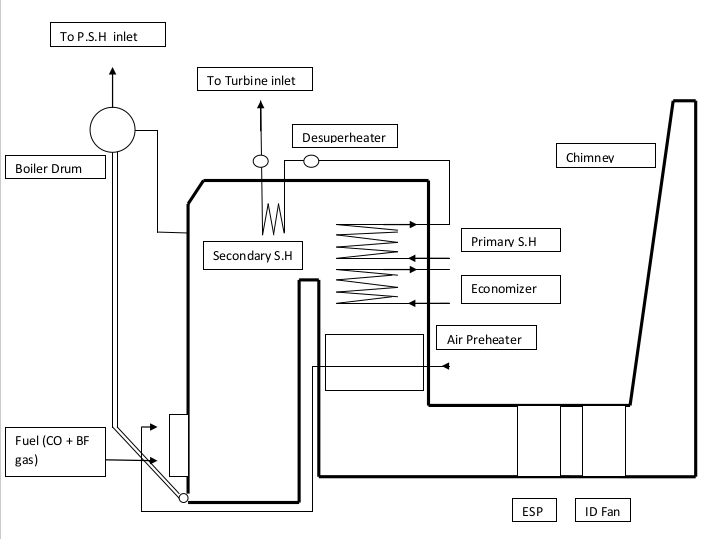
\includegraphics[width =5in]{flow}
\end{center}
    
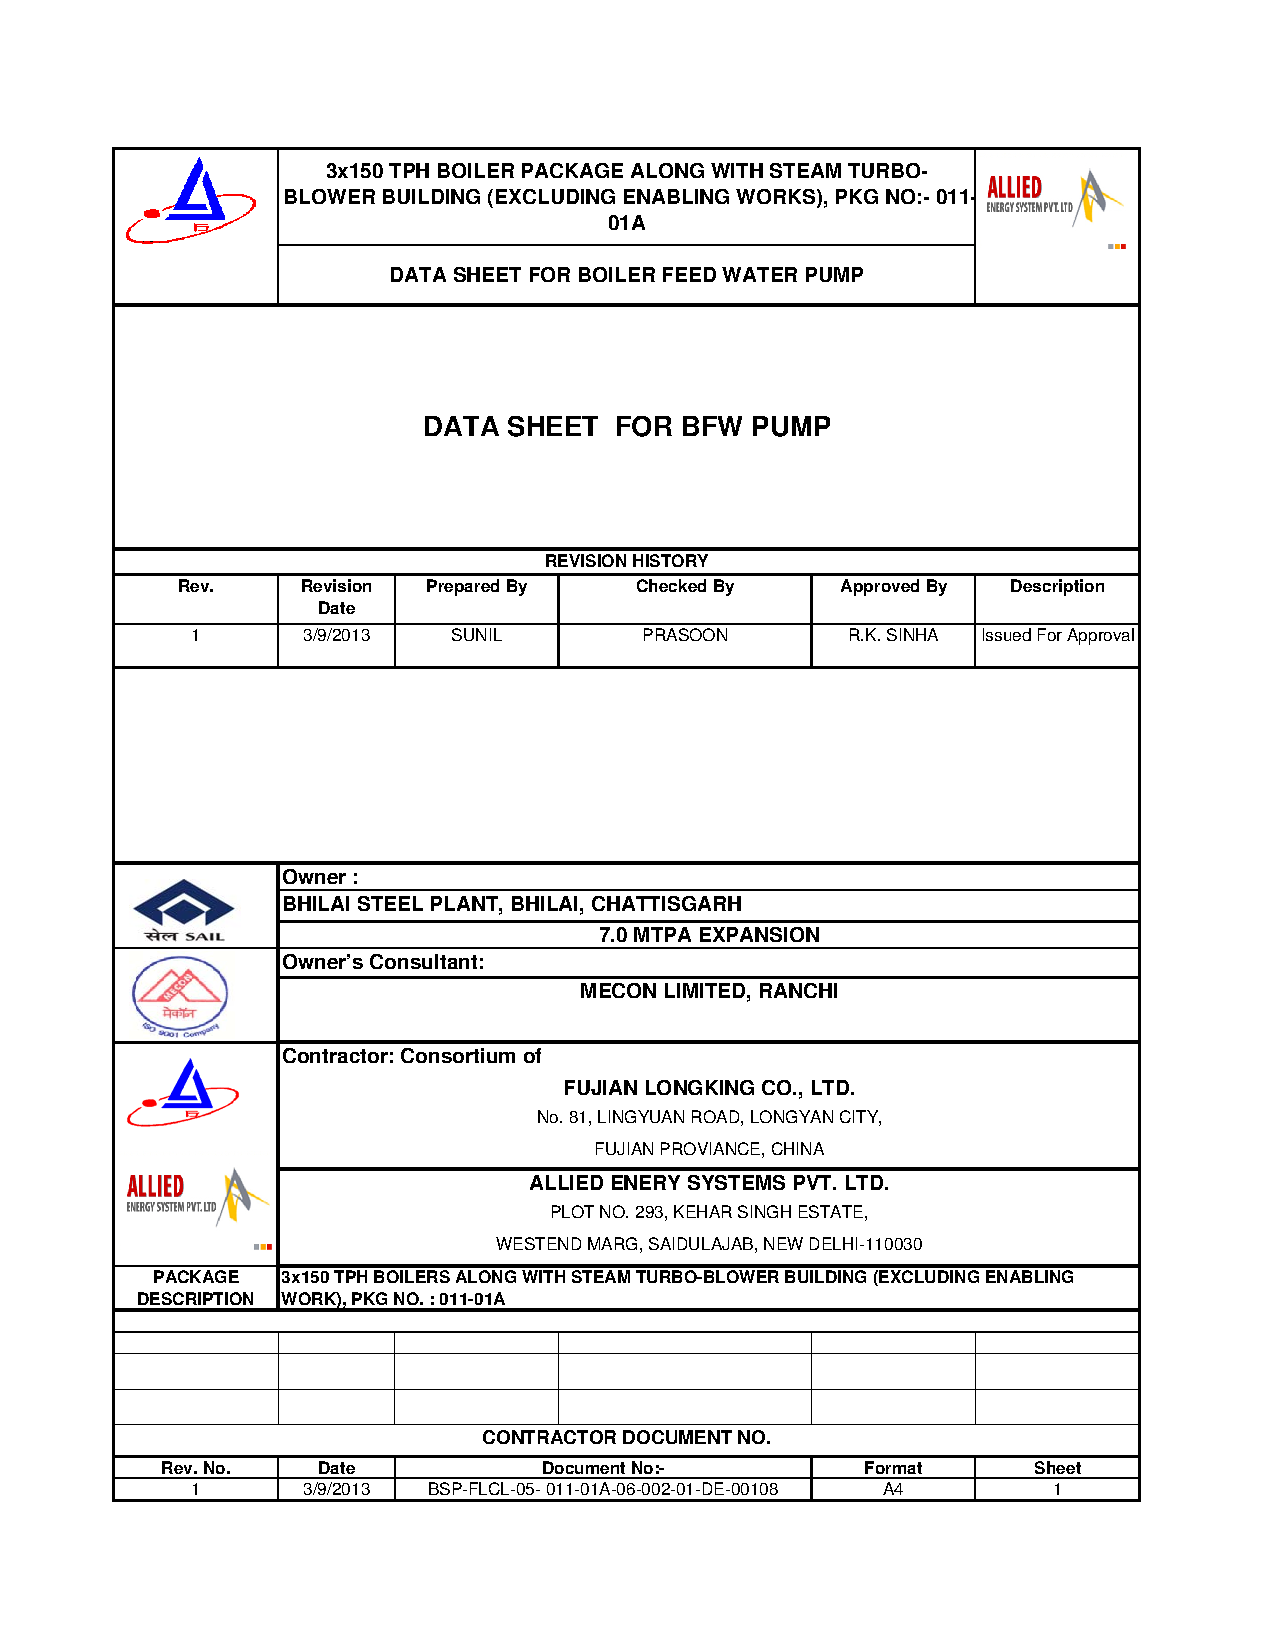
\includepdf[pages=-,angle=0]{boilerp1.pdf}
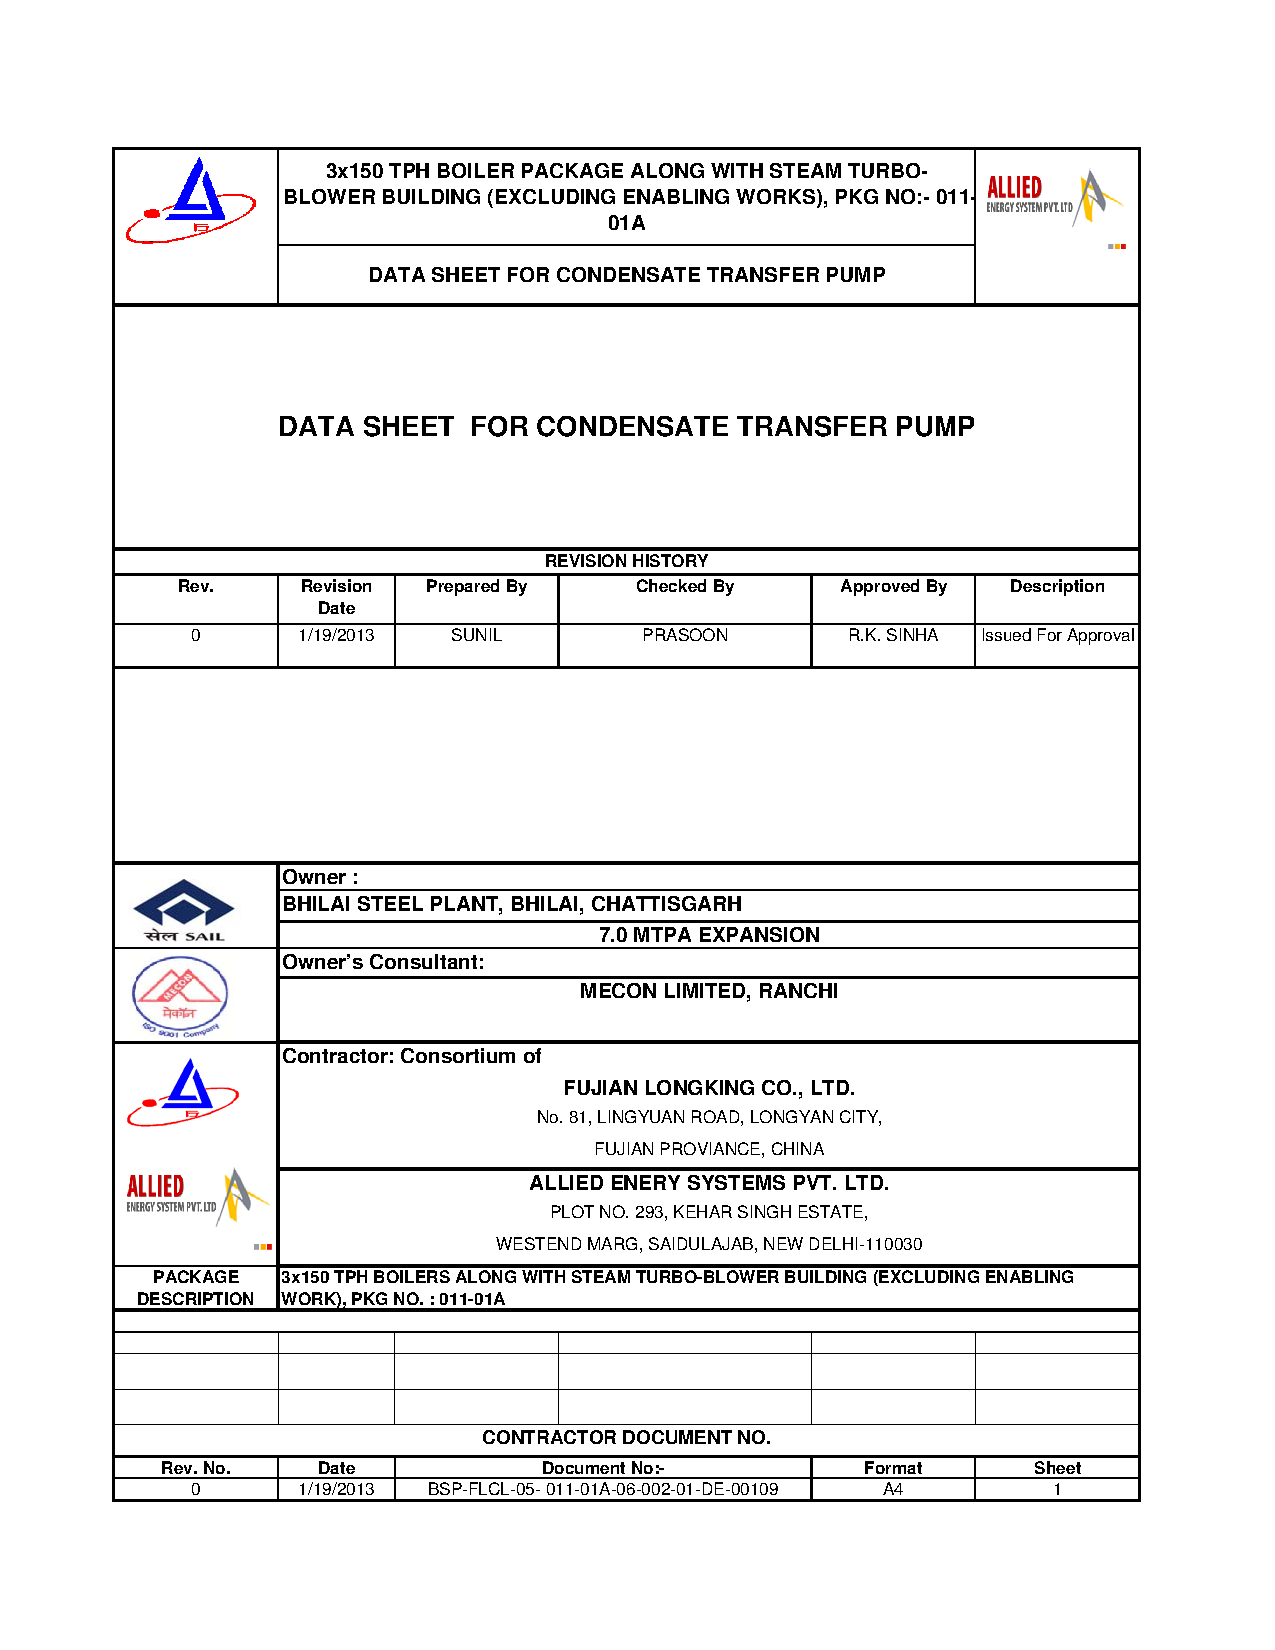
\includepdf[pages=-,angle=0]{boilerp2.pdf}
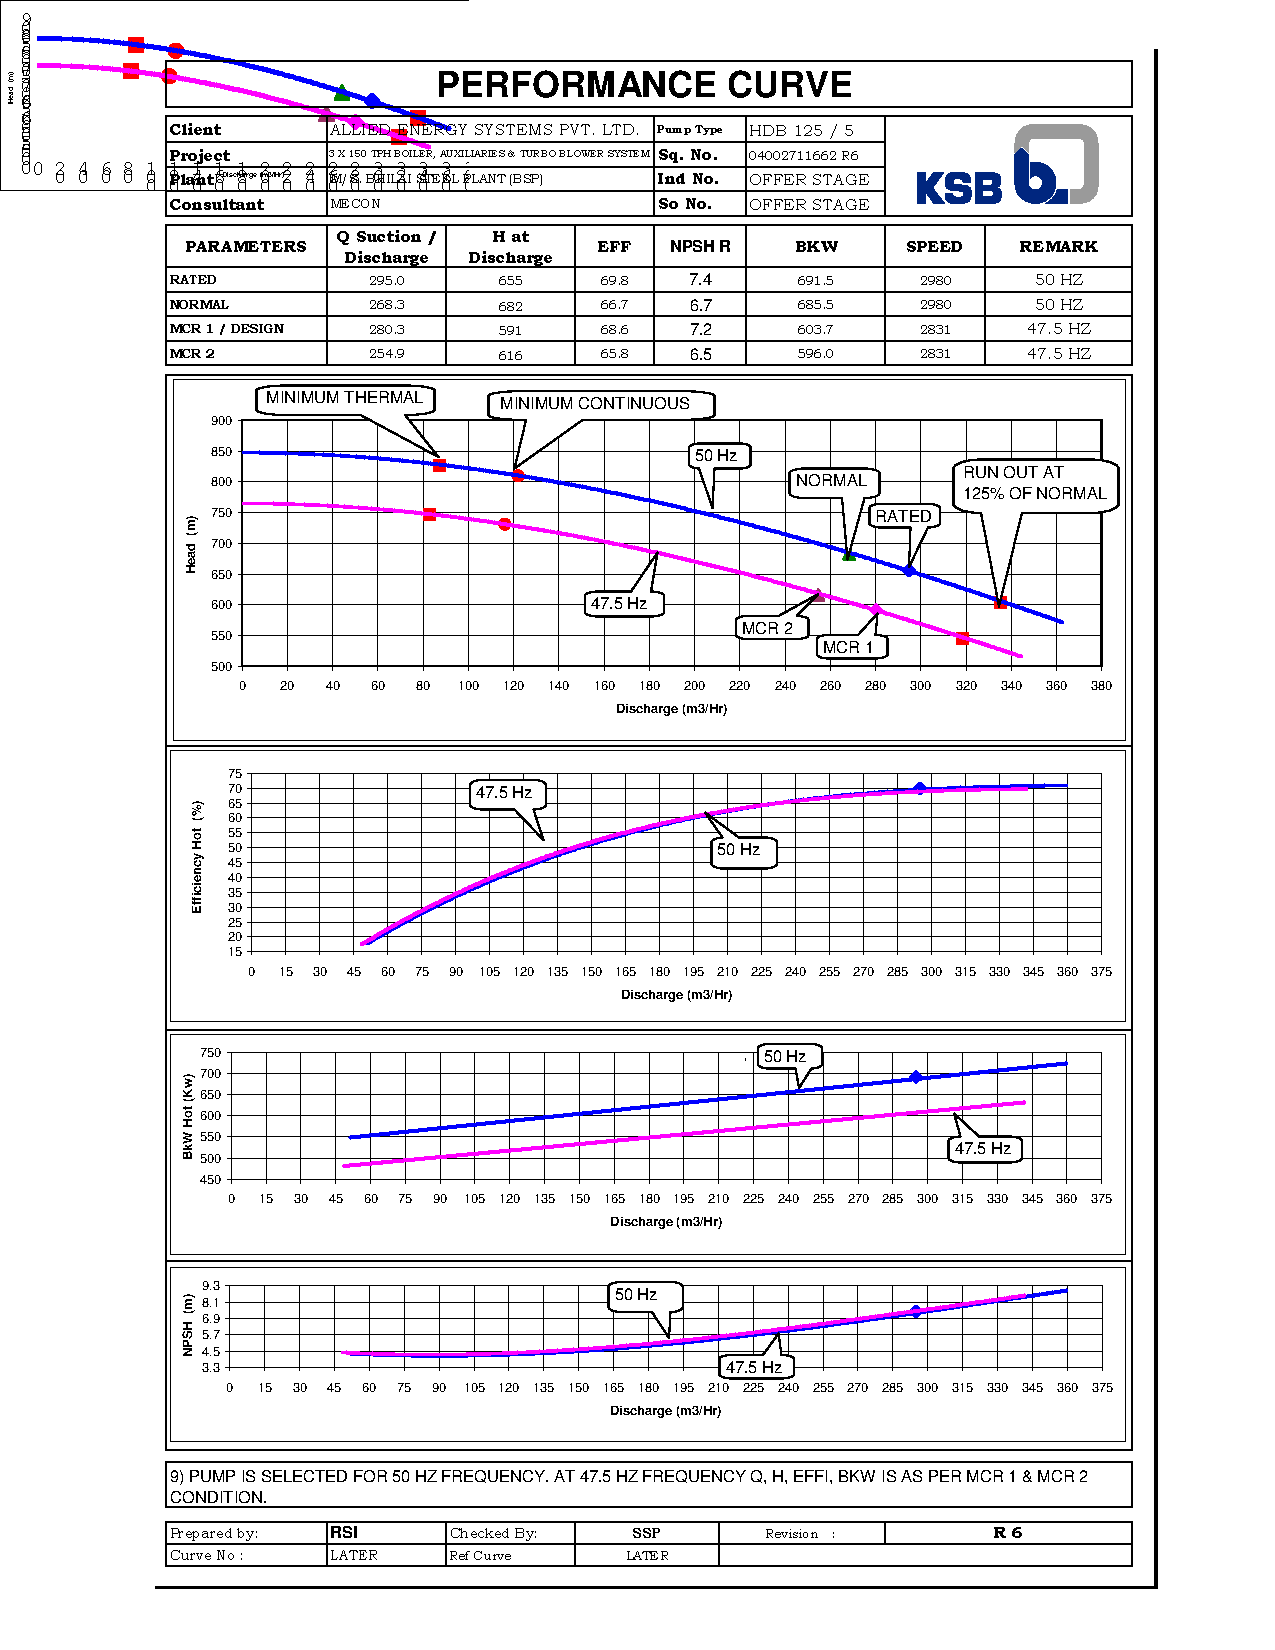
\includepdf[pages=-,angle=0]{boilerp3.pdf}
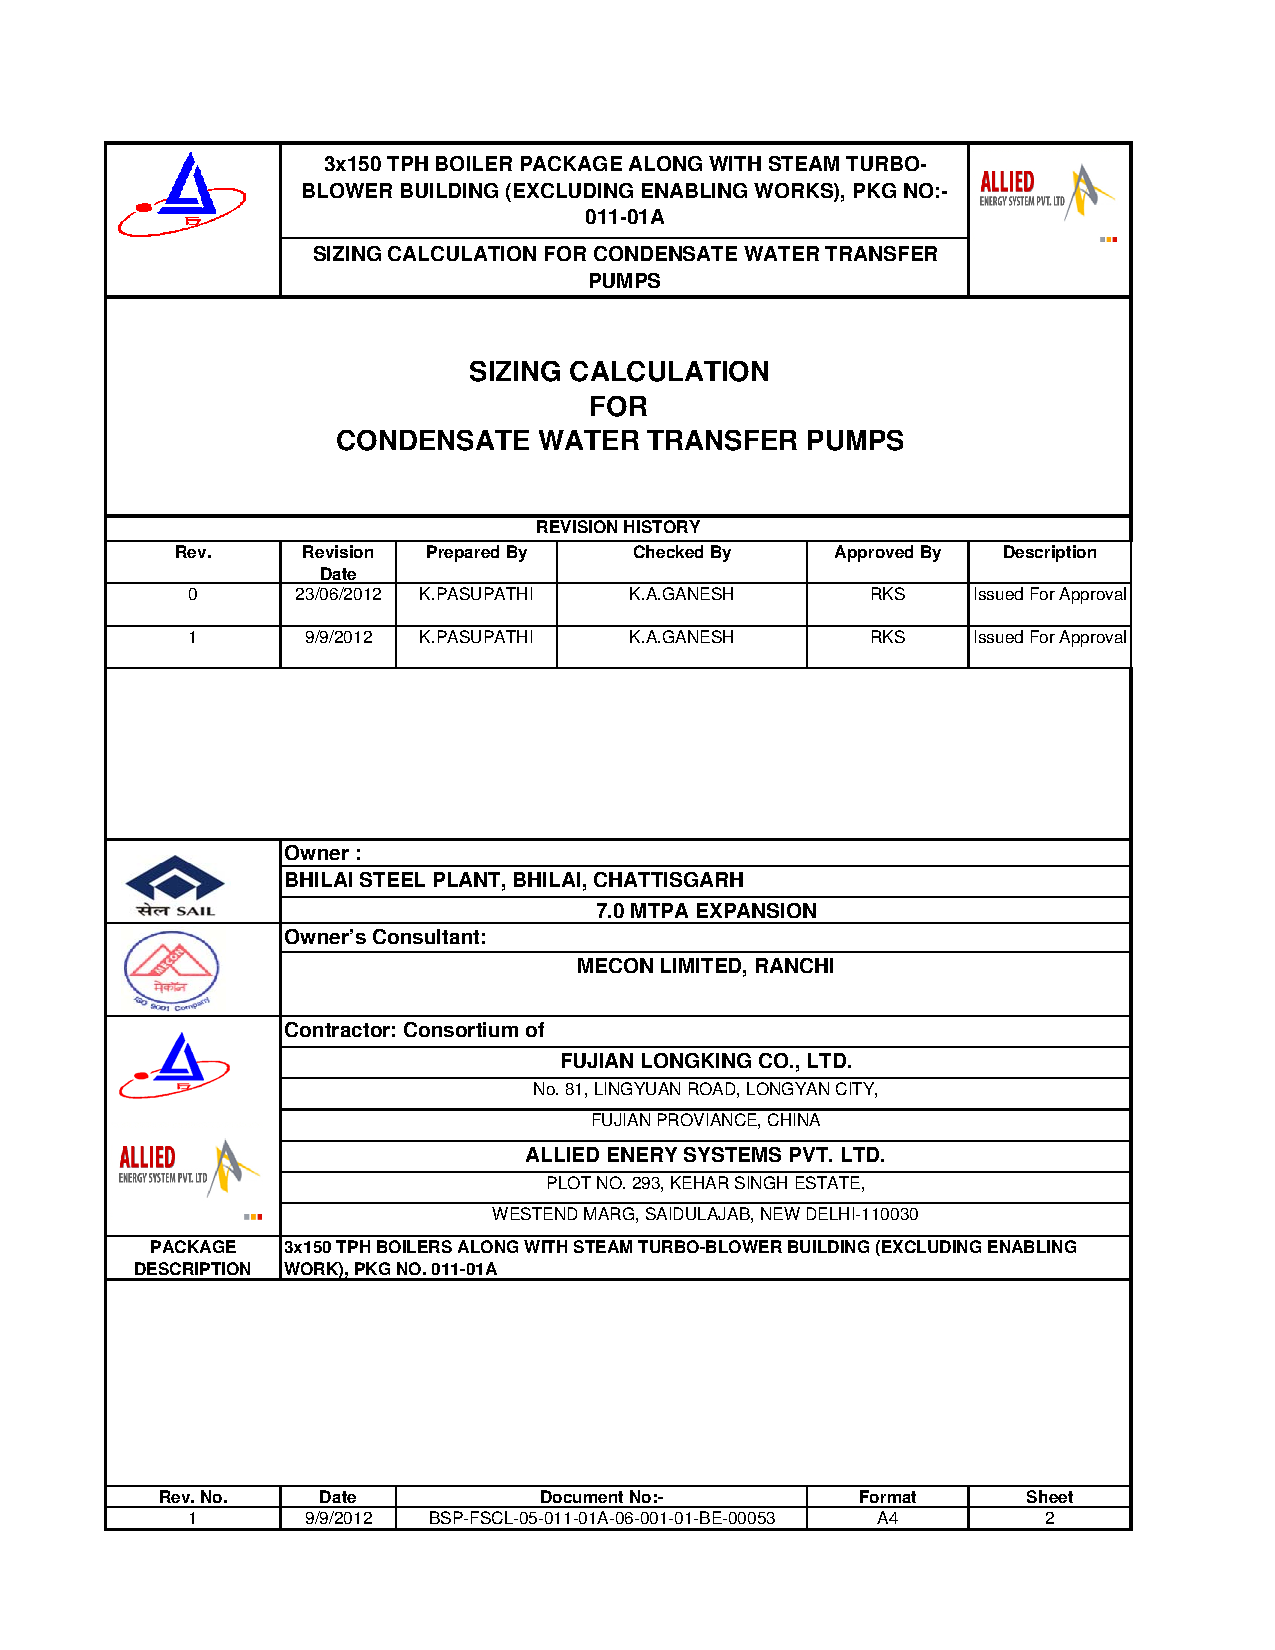
\includepdf[pages=-,angle=0]{boilerp4.pdf}
\section{Boiler and BOP Load Calculation}
\begin{center}
\begin{tabular}{|c|c|}
\hline
  BFP & 2 X 720  = 1440 kW \\ \hline
  ID Fan & 9 X 110 = 2 X 55 110 kW \\ \hline
  FD Fan & 6 X 200 = 1200 kW \\ \hline
  CTP & 2 X 150 = 300 kW\\ \hline
  Aux. Load & 700 kW \\ \hline
  Total Rated Load & 6340 kW \\ \hline
  \textbf{Act. Load(80\%)} & \textbf{5072 kW}\\
  \hline
  
\end{tabular}
\end{center}


\chapter{Steam Turbo Blowers(STB)}
\section{Need of STB in BSP}
Blast Furnaces can be considered as the heart of a Steel Plant. The blast furnace is the first step in producing steel from iron oxides. The purpose of a blast furnace is to chemically reduce and physically convert iron oxides into liquid iron called "hot metal". The raw materials such as iron ore, coke and limestone are dumped into the top and preheated air known as Hot air blast is blown into the bottom. The raw materials undergo numerous chemical reactions and descend to the bottom to become final product of liquid iron and slag. The hot air blast is produced by passing cold air blast trough a stove where residual blast furnace gases are burned. This cold air blast is provided by Turbo blowers form Power and Blowing Station. \\
Each blower installed on the new Power and Blowing station will provide on average 1500 $Nm^{3}/min$ of cold air blast. There will be 3 Steam Turbine driven Turbo Blowers (2 working and 1 Standby) each with 50\% capacity of maximum air blast requirement.\\

\section{Flow Diagram of STB and Auxiliaries}
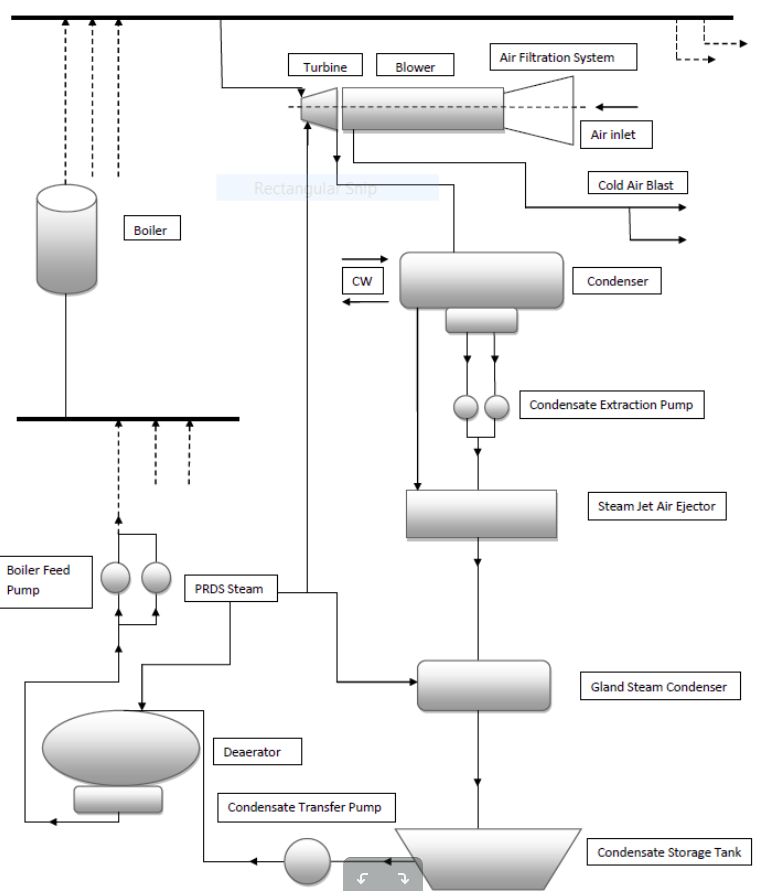
\includegraphics[width =6in]{stbflow.png}


\section{Process Overview of STB and Auxiliaries}
The steam used to drive the blowers is produced in \textbf{3 Boilers} at 40 ata, 450 degree Celsius. Waste gases from blast furnace and coke oven mainly BF gas and CO gas are used to fire the
burners in boiler to produce steam. The steam so produced is sent to main steam header from
where tapings are taken for different stations mainly \textbf{Turbo blowers, Turbo generators and
Pressure Reducing and De superheating Station}.\\[1em]
Steam enters the \textbf{Turbine} at around 36 ata, 440 degree Celsius. The steam in turbine passes
through different stages where its enthalpy is converted into rotational energy to drive the
turbine shaft which in turn drives the \textbf{Blower} attached. The blower thus sucks the air passing through air filtration system and delivers the high pressure air to the blower outlet. The steam from turbine outlet goes through \textbf{Condenser} where it is condensed by cooling water to liquid condensate which is collected in hotwell.\\[1em]
The liquid condensate from the hotwell is then pumped using \textbf{Condensate Extraction Pump}.
The condensate is then passed through the \textbf{Steam Jet Air Ejector} where the condensate is
heated and the air in the condenser is simultaneously ejected using the steam from \textbf{PRDS}. The condensate is then passed through the \textbf{Gland Steam Condenser} where it is heated using the PRDS steam.\\[1em]
The condensate is then stored in the \textbf{Condensate Storage Tank}. The condensate is then
transferred to the \textbf{Dearator} using the \textbf{Condensate Transfer Pump}. The condensate is sprayed from the top in the dearator and PRDS steam is used to heat the condensate and remove the
impurities. The feed water so formed is collected and then pumped to the Boiler using the
\textbf{Boiler Feed Pump}. The feedwater in boiler is first converted to saturated liquid by
economizer and then it goes to the boiler drum where it is evaporated and then passes through
superheater before reaching its final state and transferred to main steam header.
\section{Layout of STB PBS-2}
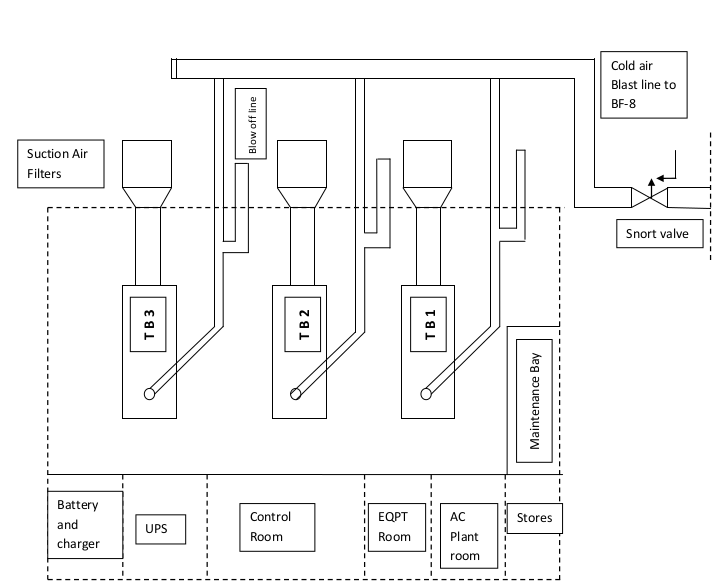
\includegraphics[width =6in]{layoutstb}
\section{Air Distribution system STB PBS-2}
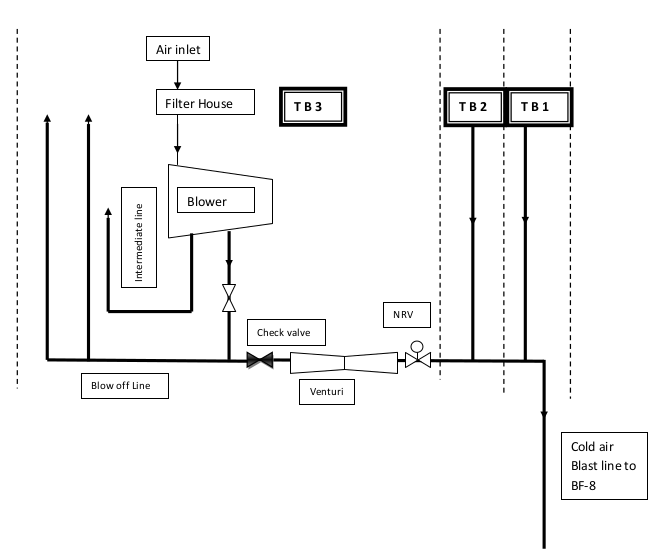
\includegraphics[width =6in]{airstb}

\section{Turbo Blowers}
\begin{figure}[h!]
 \begin{center}
  \caption{219000 Nm /hr BLOWER AT PBS-2 STB}
  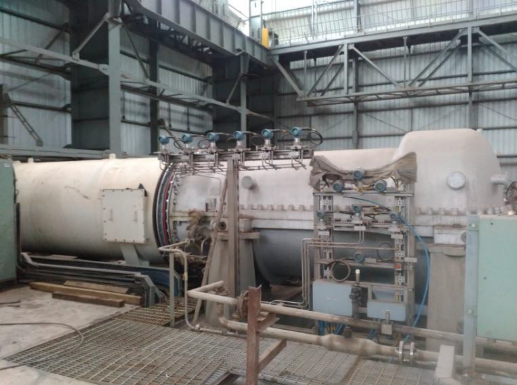
\includegraphics[width=2in]{blowerstb.png}
 \end{center}
\end{figure}\\
Turbo-blower is a combination of two turbo machines - Turbine and Blower. A turbo machine is a device that exchanges energy with a fluid using continuously flowing fluid and rotating blades The turbine is a work producing device which is run using the steam from the boilers. This turbine thus rotates the shaft attached to the blower. Blower is a work consuming device and is used to transfer energy to the fluids. Thus the turbine takes the energy from one fluid (steam) and the blower then transfers this energy to other fluid (air, in our case).\\
There are 3 ways of classifying turbo machines 
\begin{enumerate}
  \item Type of fluid they work on – Compressible or Incompressible
  \item Direction of flow in the machines – Radial, Axial or Centrifugal 
  \item Whether they deliver or extract power – Turbine or Blower 
\end{enumerate}\\


A steam turbine is a prime mover which continuously converts high pressure high temperature steam supplied by steam generator into shaft work with low temperature steam exhausted to the condenser. This energy conversion takes place in 2 steps.\\ 
High pressure high temperature steam expands in nozzle and comes out at a high velocity. The high velocity jet of steam coming out of nozzles impinge on the blades mounted on the wheel, get deflected by an angle and suffers a loss of momentum which produces torque. 
\begin{figure}[h!]
 \begin{center}
  \caption{Turbine at PBS-2 STB}
  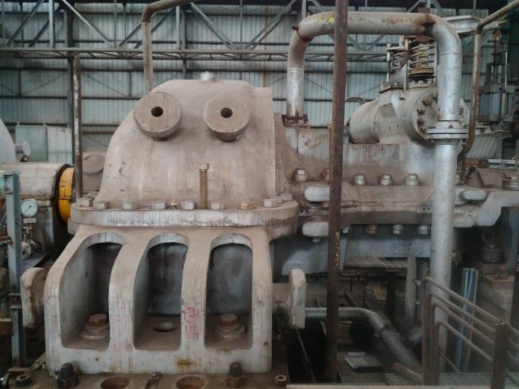
\includegraphics[width=2in]{turbinestb.png}
 \end{center}
\end{figure}
\subsection{Conservation of Mass}
Conservation of mass in simple language states that the total mass flow into the turbine equals the total mass flow out of the turbine.
$$\rho_1A_1v_1 = \rho_2A_{2}v_{2} $$
\subsection{Conservation of Momentum}
Newton’s second law applied to the rotational motion states that “Rate of change of angular momentum of a system equals the total external torque applied to the system”.
$$T = \frac{dL}{dt}$$
Also, the angular moment is given by moment of momentum
$$L = mv_\theta r$$
So the change in the angular momentum can be given as
$$mv_{2\theta}$$
and
$$T = m(v_{2\theta}r_2 - v_{1\theta}r_1)$$
And the power produced is given by
$$P = T\omega = m\omega(v_{2\theta}r_2 - v_{1\theta}r_1)$$
This is known as Euler Turbomachinery equation. This is the basic equation and applies to all
types of turbomachinery.

\section{Nozzle}
A nozzle is a duct by flowing through which the velocity of a fluid increases at the expense of pressure drop. A duct which decreases the velocity of fluid and causes a corresponding increase in pressure is called a diffuser. The shape of the nozzle depends on the mach number of a flowing fluid. If the fluid is subsonic, the nozzle will be convergent and if the flow is supersonic, the nozzle will be divergent in shape. 

\subsection{Nozzle efficiency}
Due to friction between the expansion process is irreversible, although still approximately adiabatic. In nozzle design, it is the usual practice to base all calculation on isentropic flow and then to make an allowance for friction using a coefficient or efficiency. \\
The nozzle efficiency is defined as the ratio of actual enthalpy drop to the ideal enthalpy drop.
$$ \eta_n = \frac{h_0 - h_1}{h_0 - h_{1s}} $$

\section{Blading}
Depending on the types of blade used and the method of energy transfer from the fluid to the rotor wheel, the turbine may be of two types 
\begin{itemize}
    \item Impulse turbine
    \item Reaction turbine 
\end{itemize}
In Impulse turbine, the pressure drop occurs in nozzle and no pressure drop occurs in rotors. The pressure energy is first converted to kinetic energy in nozzles and the kinetic energy is used to turn the rotor blades. These are called impulse turbines as the power is produced using the impulse of the high velocity fluid exiting the nozzles.\\
Generally, single stage turbines are not used as the enthalpy drop occurs only on one stage and the increase is velocity is very large and this results in higher blade velocity which is not desired. Hence compounding of steam turbines is necessary. The compounding is done in two ways \\
\begin{itemize}
    \item Pressure compounding or Rateau staging 
    \item Velocity compounding or Curtius staging 
\end{itemize}
\textbf{Pressure compounding} corresponds to putting a number of simple impulse stages in series. The total enthalpy drop is divided equally among the stages. 
\textbf{Velocity compounding} or curtis staging, all the pressure drop and hence enthalpy drop occurs on the single row of nozzles and the resultant kinetic energy of the steam is absorbed by the wheel in a number of rows of moving blades with stator in between the two such rows. The purpose of stator or guide blade is to guide the fluid without changing the velocity so that the fluid enters the next stage similar to the previous stage. In curtis satging as the number of rows of moving blades increases, the effectiveness of moving rows decreases.
\section{Reaction turbines}
In these turbines, the pressure drop occurs both in nozzles or fixed row of blades as well as the moving row of blades. Blades rotates both due to both the impulse effects of the jets and the reaction forces from the exiting jets on the blades and this is why they are called as reaction turbines.\\ 
The degree of reaction is defined as 
$$R = \frac{\Delta h_{rotor}}{\Delta h_{stage}}$$
The general arrangement of consist of initial two-row Curtis stage initially which involves large enthalpy drop and then remaining stages can either be of impulse type or reaction type.
\section{Blower Specification in STB PBS-2}
\begin{center}
\begin{tabular}{|c|c|}
\hline
    \textbf{Identification} &\textbf{An Air Blower} \\ \hline
    Serial Number & 6612 \\ \hline
    Vendor's Name & Man Diesel and Turbo SE \\ \hline
    Gas Handled & Air \\ \hline
    Rated Capacity & 219000 Nm^3/hr \\ \hline
    Rated Power & 22836 kW \\ \hline
    Hydrostatic Test Pressure & 10.7 kg/cm^2g \\ \hline
    Casing Design Pressure & 7.1 kg/cm^2g \\ \hline
    Casing Design Temperature & 340$^{\circ}$ \\ \hline
    Purchaser Item Number & TBB 01 \\ \hline
    Year of Fabrication & 2012 \\ \hline
    Type + Size & AG080/16RB \\ \hline
    Min. Operating Speed & 3964 rpm \\ \hline
    Max. Constant Speed & 5814 rpm \\ \hline
    Trip Speed & 6104 rpm \\ \hline
    First Critical Speed & 2663 rpm \\ \hline
    Max. allow work pressure & 7.0 kg/cm^2abs \\ \hline
    Min/Max allow temp & 9/337$^{\circ}$C \\
\hline
\end{tabular}
\end{center}

\section{Turbine Lubrication System at STB PBS-2}
The modern steam turbine and generator are carefully designed pieces of equipment constructed of well selected materials. Its satisfactory performance and useful life in service depend, among other things, on the maintenance of proper lubrication. This is one of the best insurances against turbine outage. The Lubricating oil system performs three basic functions: It reduces friction between rotating and fixed elements, It removes heat from the bearings and In mechanical hydraulic governing systems, it is used as a hydraulic pressure fluid.
Figure shows a typical turbine lubrication system. Majority of oil is stored in a Lube oil tank. Different pumps as described below take suction from pump and discharge oil for bearings. \\
\textbf{Main oil pump}\\
The main oil pump is the one that delivers all the oil requirements for the turbine-generator at high pressure during normal operation. It is direct-driven from the turbine shaft and may be located at either the turbine or generator end of the shaft. Because the main oil pump is and attached pump, it runs at turbine shaft speed. During startup and shutdown, the main oil pump is not turning fast enough to deliver the required flow so auxiliary pumps are used.\\
\textbf{Auxiliary oil pump}\\
The auxiliary oil pump has two functions. The first is to operate during the startup and shutdown when the main oil pump is not running and second is to act as a standby during the main oil pump failure. \\
\textbf{Emergency oil pump}\\ 
The time required for a turbine to run down from operating speed to a stop is typically from 20 to 45 minutes. If the bearings did not receive lubrication during this period, they would rapidly overheat and be destroyed. The only method of protection is to provide a sufficient number of alternate power supply lube oil pumps to insure all lube oil flow is not lost. The auxiliary lube oil pump is normally backed up with ac and dc emergency lube oil pump. This pump is automatically started from a pressure switch in the lube oil supply header to the bearings. \\
\textbf{Jacking oil pump }\\
When the heavy turbine-generator shaft is at rest, It will squeeze the oil film from under the shaft at the bearings. If the shaft is then rotated, there will be metal-to-metal rubbing until the oil can work its way underneath. To avoid this situation, the jacking oil pump injects oil at high pressure into the bearing at the bottom of the shaft. This tends to lift or jack the shaft a few hundredths of a millimeter off the bearing so that there will be no metal-to-metal contact.\\
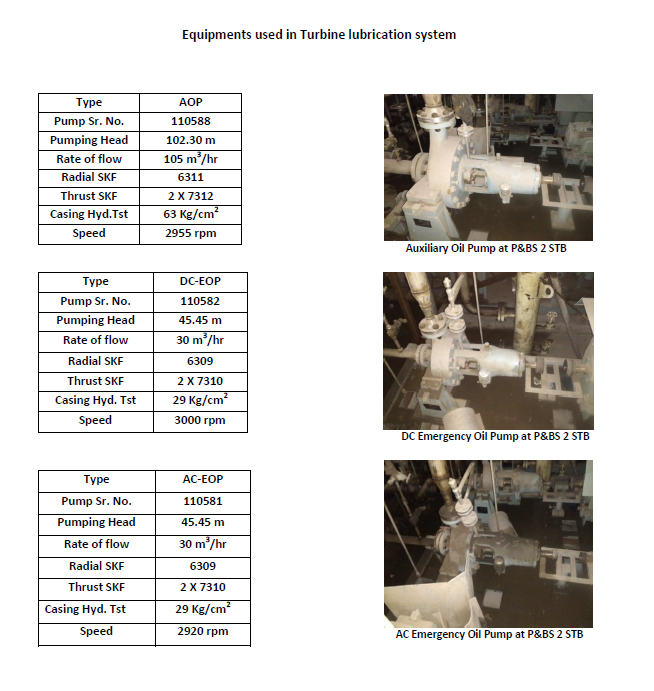
\includegraphics[width = 6in]{equip.png}
\section{Single Line Diagram}
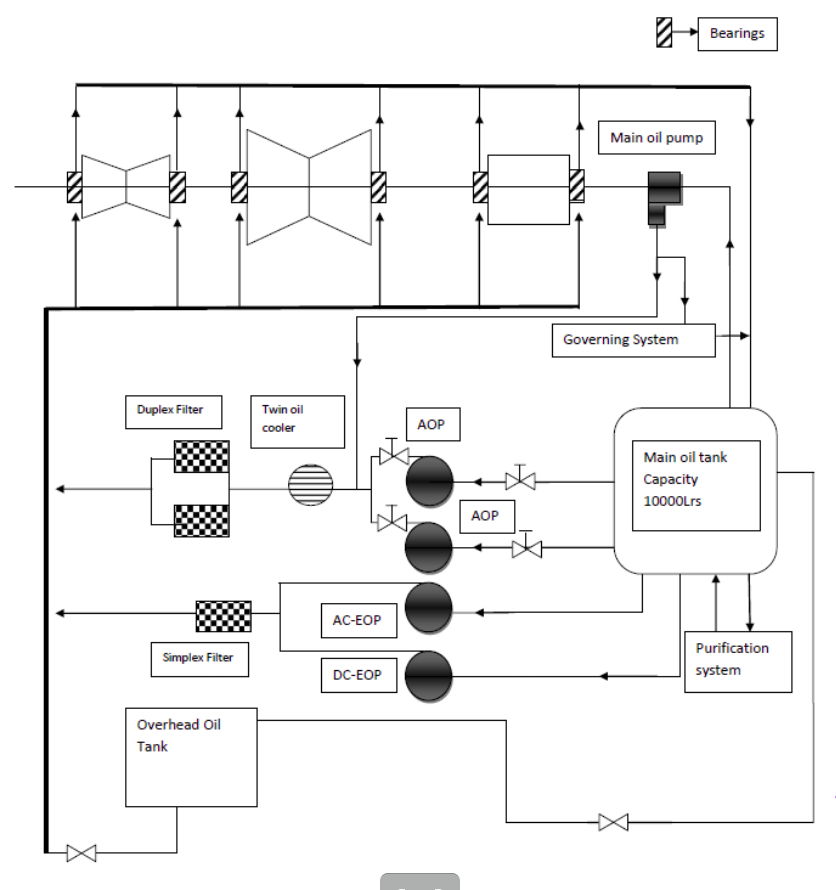
\includegraphics[width = 6in]{turbinelub.png}
\section{STB Load Calculation}
\begin{center}
\begin{tabular}{|c|c|}
\hline
  AOP & 3 X 1680 = 2 X 55 110 kW \\ \hline
  CEP & 9 X 110 = 2 X 55 110 kW \\ \hline
  Aux. Load & 400 kW \\ \hline
  Total Rated Load & 620 kW \\ \hline
  \textbf{Act. Load(80\%)} & \textbf{496 kW}\\
  \hline
  
\end{tabular}
\end{center}

\chapter{Circulating Water and Pump House}
\section{Overview}
Circulating towers are the devices that take heat from the cooling water to cool them for condenser heat removal. The heat is rejected to the atmosphere. The cooling towers can be further divided as Wet type and Dry type.
\subsection{Wet Cooling towers}
Wet cooling tower have showers that sprays hot water over horizontal packing. The outside
air enters the tower through louvers on the side of the tower. The water evaporated is
directly proportional to cooling. Cold water is collected in a concrete basin and is pumped
again to the condensers.\\[1em]
The minimum temperature to which water can be cooled is the adiabatic saturation or wet
bulb temperature of the ambient air. At this temperature, the air is 100 % saturated and
cannot absorb more moisture.\\[1em]
A Cooling tower is specified by
$$Approach(A) = (Exit \,Temperature \,of \,C.W.) - (WBT \,of \,ambient \,air)$$
where WBT stands for Wet Bulb temperatue which is the temperature a parcel of air would have if it were cooled to saturation (100\% relative humidity) by the evaporation of water into it, with the latent heat being supplied by the parcel.\\[1em]
Also the cooling efficiency is defined as
$$\eta = \frac{Actual \,Cooling}{Maximum \,possible \,Cooling}$$
We have 10 cooling cells with 9 working and 1 standby. Temperature reduces from 42$^{\circ}$ to 34$^{\circ}$ at supplied to STG and STB condensor. Its cooling capacity is 19655 m$^3$/hr. It has 5 vertical axial flow pumps with 3 working and 2 for standby. Water sump in pump house is 8.5 m deep.
\section{Diagram}
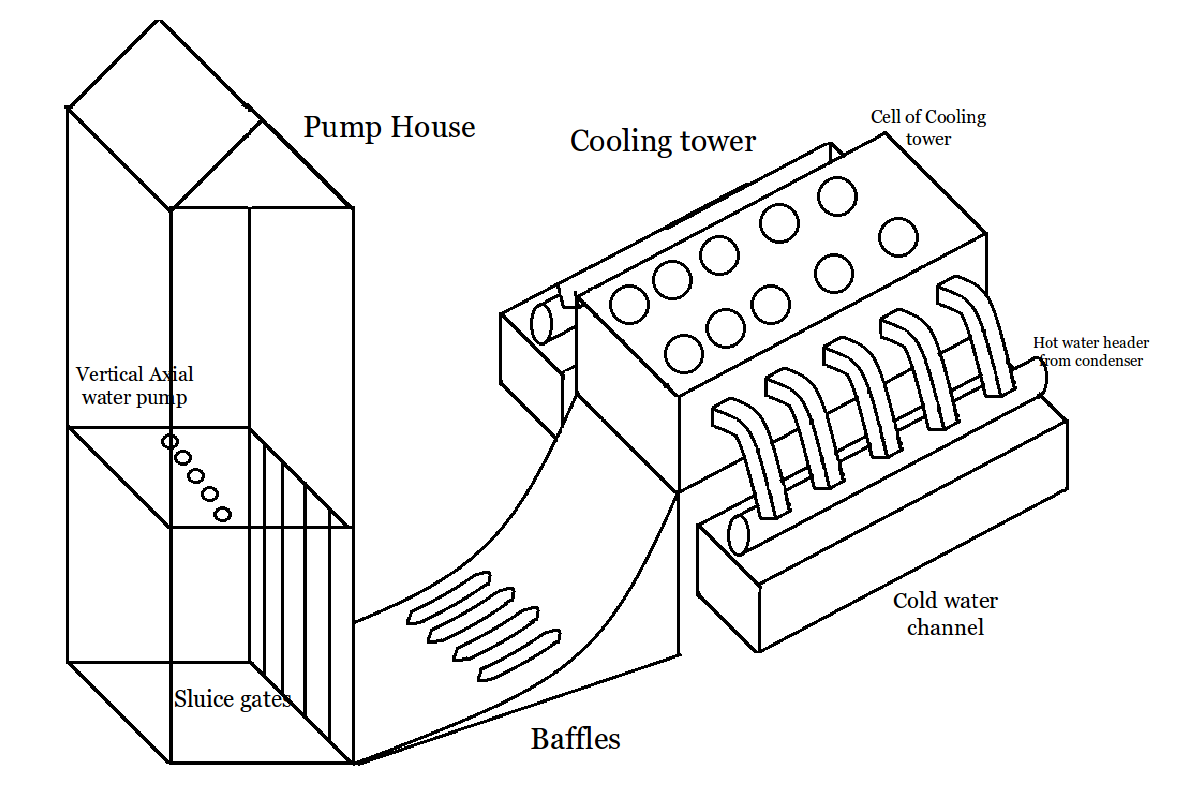
\includegraphics[width =6in]{cooling}
\section{CWPH Load Calculation}
\begin{center}
\begin{tabular}{|c|c|}
\hline
  CW Pump & 3 X 1680 = 5040 kW \\ \hline
  CT Fans & 9 X 110 = 990 kW \\ \hline
  Aux. Load & 70 kW \\ \hline
  Total Rated Load & 6100 kW \\ \hline
  \textbf{Act. Load(80\%)} & \textbf{4880 kW}\\
  \hline
  
\end{tabular}
\end{center}
\section{Single Line Diagram}
Click \href{http://i.imgur.com/cnZJrL5.png}{here} for detailed image.\\
\begin{center}
\includegraphics[width = 5in]{cwphsld.png}
\end{center}


\chapter{Conclusion}
The Power and Blowing Station is one of the most important station of Bhilai Steel Plant. The production of cold air blast is carried out in STB unit and is taken to the various blast furnaces for further conversion to the hot air blast. The waste gases from the blast furnaces and other units mainly coke oven are used as fuel to produce the cold air blast thereby reducing the fuel requirement and hence the overall efficiency of the plant. The project tries to explain various processes and equipments used in the production of cold air blast for the blast furnace. The various equipments for example Boiler, Condenser, Turbo-Blowers, Deaerator, Steam jet air ejector, lubrication system etc. have been studied.\\
From our calculations we concluded that total PBS-2 actual load is approximately \textbf{11678kW}\\
Usually there is the aim to minimize the friction losses, heat losses and drain leakage in steam lines of any power plant. Often, this is the primary goal and proper utilization of pipe length (shortest route to carry steam), proper insulation and installation of well working drain valve are favorable solution. However, in Bhilai steel plant, most of the plants use old technology, therefore only a very small proportions of waste steam is utilize including turbo blower and turbo generator condensate (initially exhauster steam also feeds back to boiler but not now).\\
At present all the consumers of PBS don’t feed condensate back to the boiler this is the biggest loss because we demineralized water for water this require a lot of input. So utilization of used steam by condensing might reduce the steam losses and will increase power plant efficiency to a remarkable extent. Insulation is the main factor in heat losses, glass wool (or mineral wool) with aluminum coating is commonly used, according to diameter of standard value of insulation is provided. But provided insulation should be repaired within a time interval but as it is seen in BSP many steam pipe lines not having proper insulation which are leading huge heat losses. Friction losses can be minimized by avoiding unnecessary bend, trap (for drain), reducer and expander in steam line.\\
This study will result in a net return to any integrated steel plant by the recovery of steam losses. Recovery of steam losses will result reduced specific fuel consumption and which lead reduced cost of fuel and substantial reduction in steam generation cost through this work i.e. proper insulation, proper trap for drain. Implementation of this solution will definitely increase overall efficiency of power plant. BSP is not too far to recover all their pipe line insulation and proper maintenance of steam line. 
\\[1em]
\begin{center}
All materials related to our project can be found on  
\href{https://github.com/him1411/ps-project-eee}{this} GitHub repository.
\\[5em]

\textbf{\textit{The end}}
\end{center}
% \chapter{STG 25 MW}
% \section{Process Flow Diagram}
% 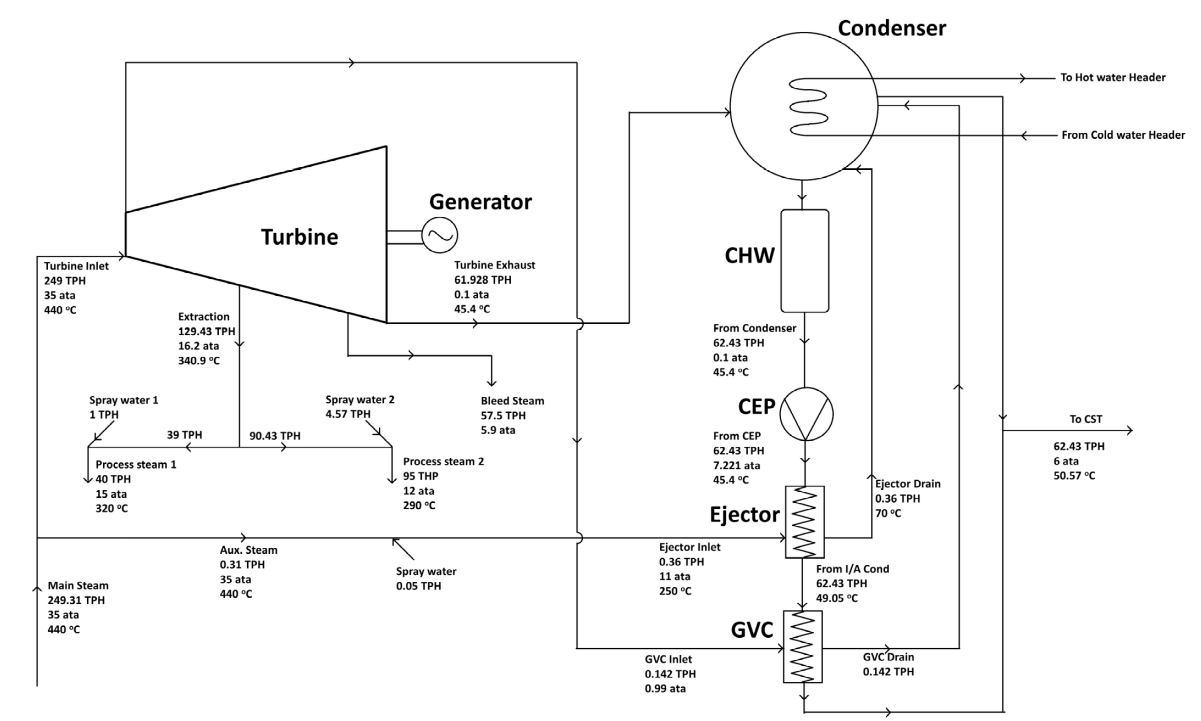
\includegraphics[width =6in]{stgprocessflow.png}
% \section{Electrical Equipment}
% \begin{center}
% \begin{tabular} { | c | c | c |} 
% \hline
% Equipment & Specification & Location \\ \hline
% Transformers & 36MVA, 11kV/6.9kV & 0 meters B-C \\ \hline
% Breakers & 1.3150 Amp, 2.2000 Amp & 11 meters A-B \\ \hline
% Reactor & 1500 Amp, 12\% & 3 meters A-B \\ \hline
% DCS &  & 11 meters \\ \hline
% LT Panels & & 11 meters\\  
% \hline
% \end{tabular}
% \end{center}
% \section{STG 25 MW Electrical Component}
% 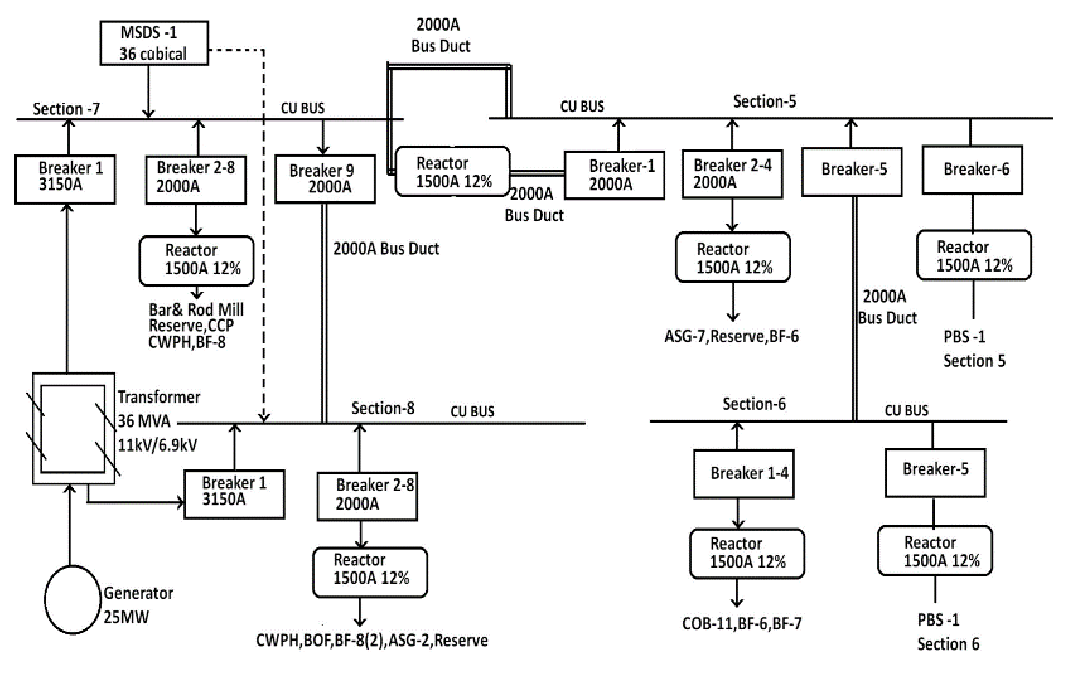
\includegraphics[width =6in]{stg25mw}
% \section{STG - Electrical Reserve Supply Switch Board}
% 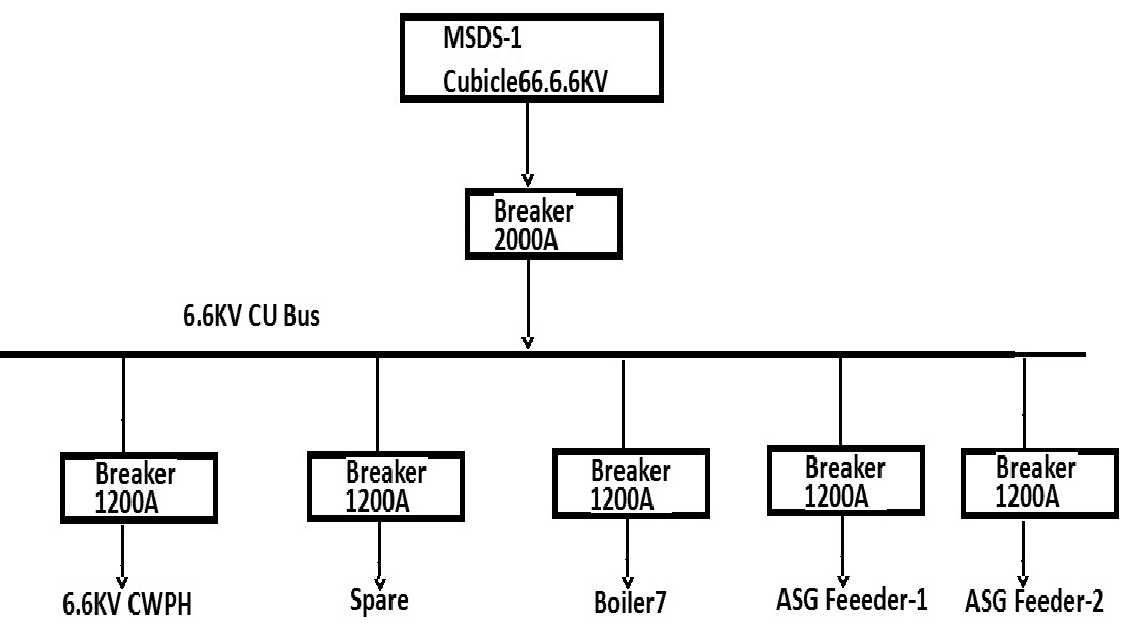
\includegraphics[width =6in]{stgelec}   

% \chapter{Cooling Tower and Pump House}
% \section{Overview}
% Cooling towers are the devices that take heat from the cooling water to cool them for condenser heat removal. The heat is rejected to the atmosphere. The cooling towers can be further divided as Wet type and Dry type.
% \subsection{Wet Cooling towers}
% Wet cooling tower have showers that sprays hot water over horizontal packing. The outside
% air enters the tower through louvers on the side of the tower. The water evaporated is
% directly proportional to cooling. Cold water is collected in a concrete basin and is pumped
% again to the condensers.\\[1em]
% The minimum temperature to which water can be cooled is the adiabatic saturation or wet
% bulb temperature of the ambient air. At this temperature, the air is 100 % saturated and
% cannot absorb more moisture.\\[1em]
% A Cooling tower is specified by
% $$Approach(A) = (Exit \,Temperature \,of \,C.W.) - (WBT \,of \,ambient \,air)$$
% where C.W. stands for Cooling Tower and WBT stands for Wet Bulb temperatue which is the temperature a parcel of air would have if it were cooled to saturation (100\% relative humidity) by the evaporation of water into it, with the latent heat being supplied by the parcel.\\[1em]
% Also the cooling efficiency is defined as
% $$\eta = \frac{Actual \,Cooling}{Maximum \,possible \,Cooling}$$
% We have 10 cooling cells with 9 working and 1 standby. Temperature reduces from 42$^{\circ}$ to 34$^{\circ}$ at supplied to STG and STB condensor. Its cooling capacity is 19655 m$^3$/hr. It has 5 vertical axial flow pumps with 3 working and 2 for standby. Water sump in pump house is 8.5 m deep.
% \section{Diagram}
% 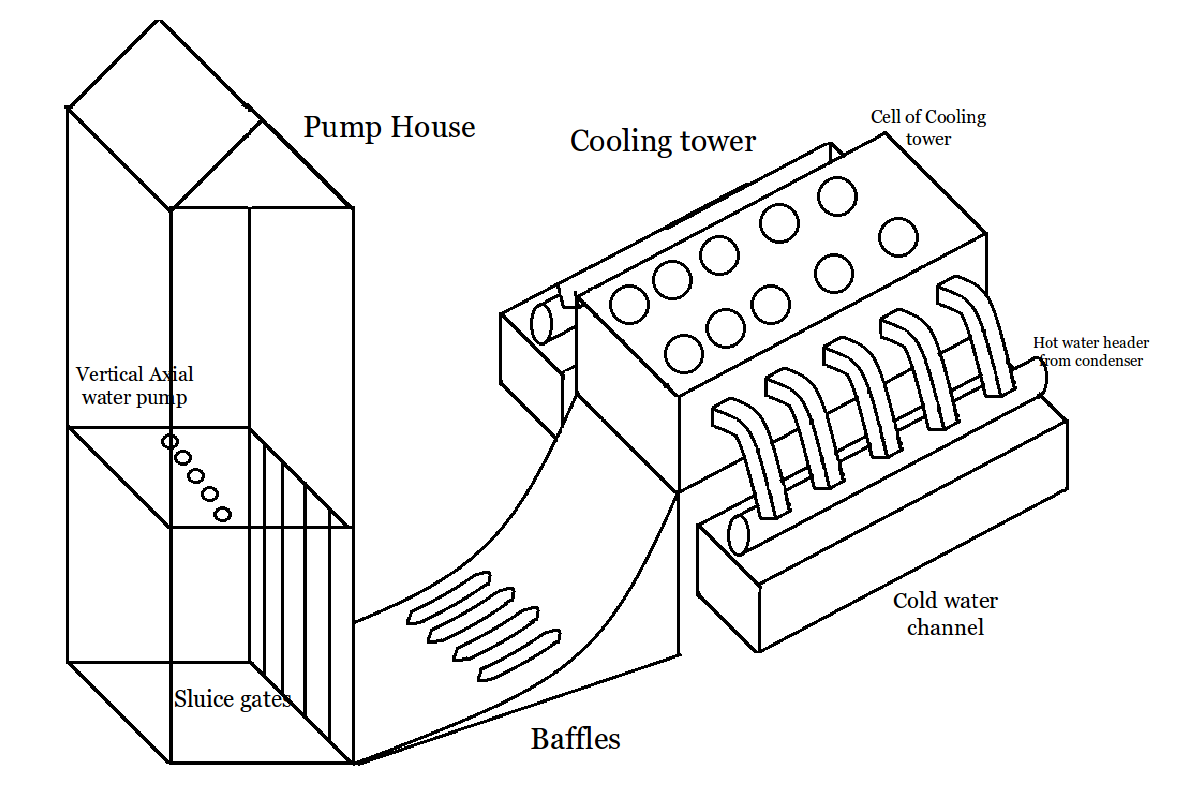
\includegraphics[width =6in]{cooling}

% \chapter{STB}
% \section{Process Overview of STB and Auxiliaries}
% The steam used to drive the blowers is produced in \textbf{3 Boilers} at 40 ata, 450 degree Celsius. Waste gases from blast furnace and coke oven mainly BF gas and CO gas are used to fire the
% burners in boiler to produce steam. The steam so produced is sent to main steam header from
% where tapings are taken for different stations mainly \textbf{Turbo blowers, Turbo generators and
% Pressure Reducing and De superheating Station}.\\[1em]
% Steam enters the \textbf{Turbine} at around 36 ata, 440 degree Celsius. The steam in turbine passes
% through different stages where its enthalpy is converted into rotational energy to drive the
% turbine shaft which in turn drives the \textbf{Blower} attached. The blower thus sucks the air passing through air filtration system and delivers the high pressure air to the blower outlet. The steam from turbine outlet goes through \textbf{Condenser} where it is condensed by cooling water to liquid condensate which is collected in hotwell.\\[1em]
% The liquid condensate from the hotwell is then pumped using \textbf{Condensate Extraction Pump}.
% The condensate is then passed through the \textbf{Steam Jet Air Ejector} where the condensate is
% heated and the air in the condenser is simultaneously ejected using the steam from \textbf{PRDS}. The condensate is then passed through the \textbf{Gland Steam Condenser} where it is heated using the PRDS steam.\\[1em]
% The condensate is then stored in the \textbf{Condensate Storage Tank}. The condensate is then
% transferred to the \textbf{Dearator} using the \textbf{Condensate Transfer Pump}. The condensate is sprayed from the top in the dearator and PRDS steam is used to heat the condensate and remove the
% impurities. The feed water so formed is collected and then pumped to the Boiler using the
% \textbf{Boiler Feed Pump}. The feedwater in boiler is first converted to saturated liquid by
% economizer and then it goes to the boiler drum where it is evaporated and then passes through
% superheater before reaching its final state and transferred to main steam header.
% \section{Layout of STB PBS-2}
% 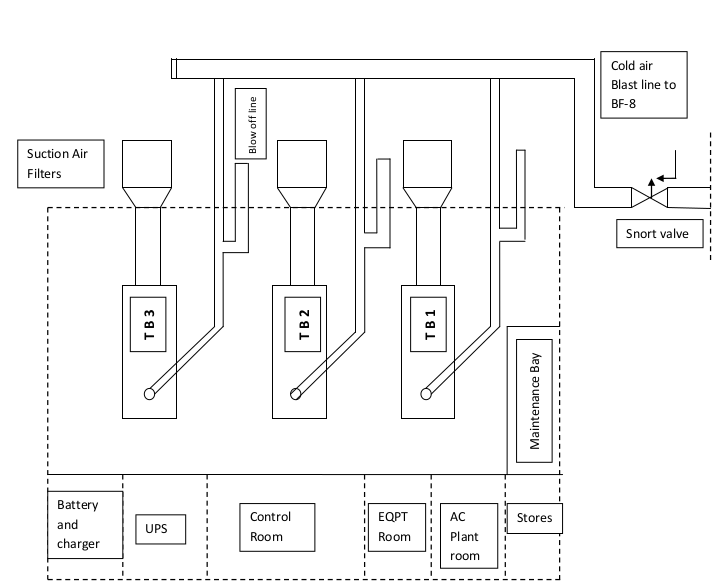
\includegraphics[width =6in]{layoutstb}
% \section{Air Distribution system STB PBS-2}
% 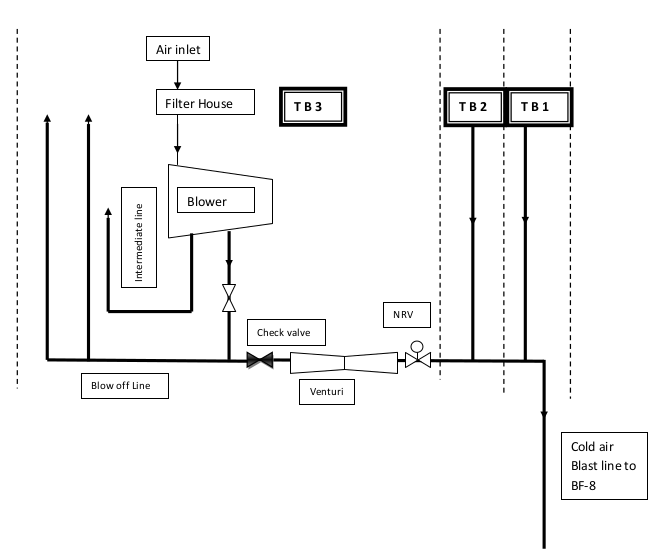
\includegraphics[width =6in]{airstb}
% \chapter{Timeline Ahead}
% \begin{tikzpicture}[snake=zigzag, line before snake = 5mm, line after snake = 5mm]
% % draw horizontal line   
% \draw (-2,0) -- (14,0);


% % draw vertical lines
% \foreach \x in {0,4,8,12}
%   \draw (\x cm,3pt) -- (\x cm,-3pt);

% % draw nodes
% % \draw (0,0) node[below=3pt] {$ 0 $} node[above=3pt] {$   $};
% % \draw (1,0) node[below=3pt] {$ 1 $} node[above=3pt] {$ 10 $};
% % \draw (2,0) node[below=3pt] {$ 2 $} node[above=3pt] {$ 20 $};
% \draw (0,0) node[below=3pt] {$ 22^{nd} June $} node[above=3pt] {$ covering \,BPTG $};
% % \draw (4,0) node[below=3pt] {$ 5 $} node[above=3pt] {$ 50 $};
% \draw (4,0) node[below=3pt] {$ covering \,STB $} node[above=3pt] {$ 24^{th} June $};
% \draw (8,0) node[below=3pt] {$ 26^{th} June $} node[above=3pt] {$ Start \,Calculations $};
% \draw (12,0) node[below=3pt] {$ Verifying \,the \,calculations $} node[above=3pt] {$ 30^{th} June $};
% \end{tikzpicture}
% \\[5em]
% \begin{center}
% \textbf{\textit{The end}}
% \end{center}

\end{document}
